\ifnum\switch=1
% -----------------------------------------------------------------------------
% ------------------------------ Extended ToC ---------------------------------
% -----------------------------------------------------------------------------

Parts of this chapter are expected to be published in:
\begin{enumerate}
\item[\cite{EchLieTic19}] \underline{C.~Echeverr{\'\i}a}, J.~Liesen, and P.~Tich{\'y}, \textbf{On the convergence of the multiplicative Schwarz~method for matrices with a special block structure}, \textbf{[Article in Preparation]}.
\end{enumerate}

\section{Introduction}
This section is based on the following references: \cite{EchLieTic19}.


\section{Differences to 1D Problems}
This section is based on the following references: \cite{EchLieSzyTic18, EchLieTic19}.


\section{The Model Problem and its Shishkin Mesh Discretization}
This section is based on the following references: \cite{GriDolSil15}.
\paragraph{Keywords:}


\section{Convergence Bounds for the Multiplicative Schwarz Method}
This section is based on the following references: \cite{EchLieSzyTic18}.


\subsection{Bounds for the Upwind Difference Scheme}


\section{Shishkin-Schwarz Preconditioning}
This section is based on the following references: \cite{EchLieTic19}.


\section{Numerical Experiments}
This section is based on the following references: \cite{EchLieTic19}.


\subsection{Poisson Problems}
This section is based on the following references: \cite{Smi85}.


\subsection{Upwind Finite Differences}
This section is based on the following references: \cite{EchLieSzyTic18, Smi85}.


\subsection{Central Finite Differences}
This section is based on the following references: \cite{EchLieSzyTic18, Smi85}.



\else
% -----------------------------------------------------------------------------
% --------------------------- Content of Chapter ------------------------------
% -----------------------------------------------------------------------------

Parts of this chapter are expected to be published in:
\begin{enumerate}
\item[\cite{EchLieTic19}] \underline{C.~Echeverr{\'\i}a}, J.~Liesen, and P.~Tich{\'y}, \textbf{Analysis of the multiplicative Schwarz~method for matrices with a special block structure.}~\textit{ [Submitted]}.
\end{enumerate}


\section{Introduction}
\label{2D:intro}
We analyze the convergence behavior of the multiplicative Schwarz method for
solving linear algebraic systems of the form
%
\begin{equation}
\label{eq:2D:linsys}
\A\u=\f,
\end{equation}
%
where the coefficient matrix $\A$ is obtained from the upwind finite difference
discretization of the two-dimensional constant coefficient convection-diffusion
equation posed on a domain $\Omega$ with Dirichlet boundary conditions
%
\begin{equation}\label{eq:2D:2Dbvp}
% \hspace*{2em}
\begin{cases}
%-\epsilon  u''(x) + \omega u'(x)+\beta u(x) = f(x), & \text{in}\; (0,1)\\
-\epsilon\left(\frac{\partial^2 u(x,y)}{\partial x^2} + \frac{\partial^2 u(x,y)}{\partial y^2}\right) + \omega_x \frac{\partial u(x,y)}{\partial x} + \omega_y \frac{\partial u(x,y)}{\partial y}+ \beta u(x,y)=f(x,y), & \text{in}\; \Omega\\
\hspace{0.8cm} u(x,y)=g(x,y),\;\text{ on }\;\partial\Omega. &
\end{cases}
\end{equation}
%
We assume
%\td{\textbf{Jorg:} In general, it needs to be carefully checked which assumptions on the model problems, discretizations, and matrices are to be made so that everything is consistent}
that the domain of definition of the BVP is the unit square, i.e.,
$\Omega=(0,1)\times(0,1)$ and further assume that the parameters of the problem
are chosen such that the the problem is \emph{convection dominated}, i.e., that
$\epsilon\ll \|\om\|$, and that the solution, $u(x,y)$, presents
\emph{one boundary layer} near $y=1$
%\td{\textbf{Jorg:} Is some condition on $\omega_x$ and $\omega_y$ known when this happens? Note that after (2.22) you assume that $\omega=[0, \omega_y]$.}.
In particular we assume that the components of the velocity field fulfill $\om=[0,\omega_y]^T$ with $\omega_y>0$, and that the scalar reaction parameter, $\beta$, is nonnegative, i.e., $\beta \geq 0$.

In order to obtain a satisfactory approximation to the solution
of~\eqref{eq:2D:2Dbvp}, we discretize $\Omega$ using a Shishkin mesh that is
refined inside the layer; a very similar approach to the one used in the
one-dimensional case (see Chapter~\ref{ch:1D}). The mesh is constructed by
using a uniform mesh in the  $x$-direction and a one-dimensional Shishkin mesh
in the $y$-direction. This technique has been described in detail in
Chapter~\ref{ch:back}, for external  sources see the
articles~\cite[\S~5]{Sty05} and~\cite{KopOri10}, as well as the
book~\cite{MilOriShi96}.
%
%By making the assumptions that $\alpha$, $\beta$, and $f$ are sufficiently
%smooth and that $\beta(x,y)-\frac{1}{2}\nabla \cdot \alpha(x,y)\geq C_0>0$ on
%$\overline{\Omega}$ for some constant $C_0$, we ensure that \eqref{eq:bvp} has
%a unique solution in the Sobolev space $H_0^1(\Omega)\cap H^2(\Omega)$ for all
%functions $f\in L^2(\Omega)$ \cite{FraLiuRooStyZho09}.
%
After the discretization process, the coefficient matrix exhibits the general
structure:

\begin{equation}
\label{eq:2D:blockmat}
\A=\left[
  \begin{array}{ccc}
             \matAHhat       & \e_{m}\otimes\matBH   &    0            \\
    \e_{m}^{\Tr}\otimes\matC  &   \matA      & \e_{1}^{\Tr}\otimes\matB \\
                   0         & \e_{1}\otimes\matCh &        \matAhhat  \\
  \end{array}
\right]\;\in\;{\mathbb R}^{N(2m+1)\times N(2m+1)},
\end{equation}
%
with the blocks $\matAHhat, \matAhhat \in \mathbb{R}^{Nm\times Nm}$,
$\matA, \matB, \matC, \matBH, \matCh \in \mathbb{R}^{N\times N}$, and
the canonical basis vectors $\e_1,\e_m\in\mathbb{R}^{m}$. We will think of
$\matAHhat, \matAhhat \in \mathbb{R}^{Nm\times Nm}$ as matrices consisting of
$m$ blocks of size $N\times N$.

It is important to note that a structure such as the one given by
\eqref{eq:2D:blockmat} is \emph{not} exclusive to the discretization of
convection-diffusion problems of type \eqref{eq:2D:2Dbvp}. The coefficient
matrices of linear algebraic systems with the structure \eqref{eq:2D:blockmat}
arise naturally when a general second-order partial differential equation is
posed and discretized inside a domain $\Omega$ that is divided by one interface
boundary into two local subdomains, $\Omega_1$ and $\Omega_2$ such as the one
shown in Figure~\ref{fig:back:shmesh2Da}.
% as shown in Figure~\ref{fig:domain}.
In this context the first $m$ block rows in the matrix $\A$ correspond
to the unknowns in the domain $\Omega_1$, the last $m$ block rows correspond to
the unknowns in the domain $\Omega_2$, and the middle block row corresponds to
the unknowns in the interface boundary. The underlying assumption here is that
in each of the two domains we have the same number of unknowns. This assumption
is made for simplicity of the following exposition. Extensions to other block
sizes are certainly possible, but would require even more technicalities.

In this chapter, after deriving general expressions for the norms of
the multiplicative Schwarz iteration matrices for systems of the form
\eqref{eq:2D:linsys}--\eqref{eq:2D:blockmat}, we derive quantitative error
bounds only for the case when the blocks $\matAHhat$ and $\matAhhat$ of $\A$ are
block tridiagonal. We point out that the model problem studied in
Chapter~\ref{ch:1D} is of the form \eqref{eq:2D:linsys}--\eqref{eq:2D:blockmat}
with $N=1$. The transition to the higher dimensional cases is reflected in the
block structure exhibited by the coefficient matrices.
While results that exploit the classical property of diagonal dominance
of tridiagonal matrices are the main tools used in Chapter~\ref{ch:1D} to
obtain quantitative convergence results, the derivation of error bounds in this
context relies on recent results on the theory of block diagonal dominance of
block tridiagonal matrices presented in Chapter~\ref{ch:BDiDo}.
% \td{\textbf{write:} add a paragraph which talks about the differences to the 1D problem treated in CH3 and BDiDo.}

The chapter is organized as follows. In Section~\ref{2D:bounds} we state the
multiplicative Schwarz method for linear algebraic systems of the form
\eqref{eq:2D:linsys}--\eqref{eq:2D:blockmat}. We continue by studying the
algebraic structure and the norm of the iteration matrices and present the main
differences to the one-dimensional case in Section~\ref{2D:bounds:structure}.
In Section~\ref{2D:bounds:convergence} we present a general expression for the
convergence factor of the method when used to solve systems with matrices of
type \eqref{eq:2D:blockmat}. We proceed by deriving quantitative error bounds
for the method when the matrix $\A$ is both block tridiagonal and
block diagonally dominant in Sections~\ref{2D:bounds:row}--\ref{2D:bounds:rowcol}. Theoretical results specific to the case of
convection-diffusion problems of type \eqref{eq:2D:2Dbvp} are given in
Section~\ref{2D:bounds:conv-diff} and numerical experiments for specific cases
are found in Section~\ref{2D:numerics}. Finally, a summary of the
main results of the chapter and a brief discussion of possible generalizations
and alternative applications of our approach is given in Chapter~\ref{ch:end}.

\newpage
\section{Convergence Bounds for the Multiplicative Schwarz Method}
\label{2D:bounds}
The multiplicative Schwarz method for solving linear algebraic systems of the
form \eqref{eq:2D:linsys}--\eqref{eq:2D:blockmat} can naturally be based on two local
solves using the top and the bottom $N(m+1)\times N(m+1)$ blocks of $\A$,
respectively. More precisely, the restriction operators of the method are given
by
\[
\R_1 \equiv \left[ \I_{N(m+1)} \quad 0 \right]
\quad \mbox{and} \quad
\R_2 \equiv \left[ 0 \quad \I_{N(m+1)} \right],
\]
both of size $N(m+1)\times N(2m+1)$. The corresponding restrictions of the
matrix $\A$ to each local subdomain (commonly refered to as \textit{local subdomain problems})are then given by
%
\begin{equation}\label{eq:2D:localsub}
\A_1 \equiv \R_1\A \R_1^{\Tr}=
\left[
\begin{array}{cc}
          \matAHhat      &  \e_{m} \otimes \matBH \\
\e_{m}^{\Tr} \otimes \C  &             \matA
\end{array}
\right], \quad
\A_2 \equiv \R_2\A \R_2^{\Tr}=
\left[
\begin{array}{cc}
            \matA       &  \e_{1}^{\Tr} \otimes \matB \\
\e_{1} \otimes \matCh   &       \matAhhat
\end{array}
\right],
\end{equation}
%
both of size $N(m+1)\times N(m+1)$. Analogous to the one dimensional case we
define the projection matrices
%
\begin{equation}\label{eq:2D:Proj}
\P_i\equiv \R_i^{\Tr}\A_i^{-1}\R_i\A\;\in\;
\mathbb{R}^{N(2m+1)\times N(2m+1)},
\quad i=1,2,
\end{equation}
%
and note that they are now of size ${N(2m+1)\times N(2m+1)}$. Once again, using
the complimentary projections
%
$$\Q_i\equiv \I-\P_i\;\in\;\mathbb{R}^{N(2m+1)\times N(2m+1)},\quad i=1,2,$$
%
we define the multiplicative Schwarz iteration matrices
%
\begin{equation}\label{eq:2D:Tij}
\T_{12}\equiv \Q_2\Q_1\quad\mbox{and}\quad \T_{21}\equiv \Q_1\Q_2.
\end{equation}
Using these iteration matrices, the method is then given by
\eqref{eq:back:schwarz}-\eqref{eq:back:error}, i.e., the transition to higher
dimensional cases is reflected only by the specific block structure of the
matrices \eqref{eq:2D:Tij}. Using the theory developed in
Chapter~\ref{ch:BDiDo} allows us to present an analogous analysis to the one
given in Chapter~\ref{ch:1D} for the one-dimensional case.

\subsection{Structure of the iteration matrices}
\label{2D:bounds:structure}
%
We begin by taking a closer look at the structure of the iteration matrices
$\T_{ij}$ in \eqref{eq:2D:Tij}. A direct computation based on \eqref{eq:2D:Proj}
shows that
%
\begin{equation*}
\P_1 =
\left[ \begin{array}{c}
\I_{N(m+1)} \\
    0
\end{array} \right]
\A_1^{-1}
\left[ \begin{array}{c|c|c}
\A_1 & \e_{m+1}\otimes \B & 0
\end{array} \right]
=
\left[\begin{array}{ccc}
\I_{N(m+1)} & \A_1^{-1}(\e_{m+1}\otimes \B) & 0\\
  0    &                  0                 & 0
\end{array}\right],\nonumber
\end{equation*}
%
and
%
\begin{equation*}
\P_2 =
\left[\begin{array}{c}
    0    \\
\I_{N (m+1)}
\end{array}\right]
\A_2^{-1}
\left[\begin{array}{c|c|c}
 0 &  \e_{1}\otimes \C & \A_2
\end{array}\right]
=
\left[\begin{array}{ccc}
0 &           0                         & 0       \\
0 & \A_2^{-1}(\e_{1}\otimes \C) & \I_{N (m+1)}
\end{array}\right],\nonumber
\end{equation*}
%
where $\e_1,\e_{m+1}\in{\mathbb R}^{m+1}$. We see that both $\P_1$ and $\P_2$
have exactly $N(m+1)$ linearly independent columns, and hence
%
\begin{equation*}%\label{eq:rankrelation}
\mathrm{rank}(\P_1) = \mathrm{rank}(\P_2)=N(m+1).
\end{equation*}
%
Moreover, the complementary projections are
%
\begin{equation*}
\Q_1  =
\left[
  \begin{array}{ccc}
    0 & -\A_1^{-1}(\e_{m+1}\otimes \B)  & 0 \\
    0 & \I_{N}                            & 0 \\
    0 & 0                                & \I_{N(m-1)}
  \end{array}
\right],\;\;
\Q_2  =
\left[
  \begin{array}{ccc}
    \I_{N(m-1)} & 0                             & 0 \\
    0          & \I_{N}                         & 0 \\
    0          & -\A_2^{-1}(e_{1}\otimes \C) & 0
  \end{array}
\right],
\end{equation*}
%
and we have
%
\begin{equation*}%\label{eq:rankrelation}
\mathrm{rank}(\Q_1) = \mathrm{rank}(\Q_2)=Nm.
\end{equation*}
%
In order to simplify the notation we write
%
\begin{equation}\label{eq:2D:pi_and_p}
\left[
  \begin{array}{c}
    \POne \\ \PiOne
  \end{array}
\right]
\equiv
\A_1^{-1}(\e_{m+1}\otimes \B)%\in\mathbb{R}^{N(m+1)\times N}
\quad\mathrm{and}\quad
\left[
  \begin{array}{c}
    \PiTwo \\ \PTwo
  \end{array}
\right]
\equiv
\A_2^{-1}(\e_{1}\otimes \C),
\end{equation}
%
where $\mathbf{\Pi}^{\klein{(i)}} \in \mathbb{R}^{N\times N}$, and
%
\begin{equation*}
\P^{\klein{(i)}} =
\left[\left(\P_1^{\klein{(i)}}\right)^{\Tr},\ldots,
\left(\P_{m}^{\klein{(i)}}\right)^{\Tr}\right]^{\Tr}
\in \mathbb{R}^{Nm\times N}\quad\mathrm{with}\quad \P^{\klein{(i)}}_j
\in \mathbb{R}^{N\times N},\;\mathrm{for}\;j=1,\dots,m.
\end{equation*}
%
Then
%
\begin{align*}
\Q_1 & =
\left[\begin{array}{c c c c}
             0_{Nm} &     & -\POne     &             \\%\hline
                 & 0_N & -\PiOne        &             \\%\hline
                 &     &      \I_N       &             \\%\hline
                 &     &                & \I_{N (m-1)}
      \end{array}\right],\quad
%
%\left[\begin{array}{c|c|c|c|c}
%0_{N(m-1)}  &     &     & -\POne_{1:m-1} &             \\\hline
%            & 0_N &     & -\POne_{m}     &             \\\hline
%            &     & 0_N & -\PiOne        &             \\\hline
%            &     &     &      I_N       &             \\\hline
%            &     &     &                & I_{N (m-1)}
%\end{array}\right],\\
\Q_2 =
\left[\begin{array}{c c c c}
\I_{N(m-1)}  &                &     &                 \\%\hline
            & \I_N            &     &                 \\%\hline
            & -\PiTwo        & 0_N &                 \\%\hline
            & -\PTwo         &     & 0_{Nm}
\end{array}\right],
%
%\left[\begin{array}{c|c|c|c|c}
%I_{N(m-1)}  &                &     &     &            \\\hline
%            & I_N            &     &     &            \\\hline
%            & -\PiTwo        & 0_N &     &            \\\hline
%            & -\PTwo_{1}     &     & 0_N &            \\\hline
%            & -\PTwo_{2:m}   &     &     & 0_{N(m-1)}
%\end{array}\right],
\end{align*}
%
and these matrices yield
%
\begin{align} \label{eq:2D:T12}
\T_{12}&=\Q_2\Q_1 =
\left[
  \begin{array}{ccc}
    0  &      -\POne               &  0     \\
    0  & \PiTwo \POne_{m}          &  0     \\
    0  & \PTwo \POne_{m} &  0
  \end{array}
\right] \\
 &=\left[
  \begin{array}{c}
    -\POne                  \\
	  \PiTwo\POne_{m}   \\
	  \PTwo \POne_{m}  \\
  \end{array}
\right]
\left[
  \begin{array}{c|c|c}-
    0_{N(m+1)} & \I_N & 0_{N(m-1)}
  \end{array}
\right]
\equiv \V_1(\e_{m+2}^{\Tr}\otimes \I_N), \nonumber
\end{align}
%
and
%
\begin{align} \label{eq:2D:T21}
\T_{21}&=\Q_1\Q_2 =
\left[
  \begin{array}{ccc}
    0  &  \POne \PTwo_{1}  &  0     \\
    0  & \PiOne\PTwo_{1}           &  0     \\
    0  &  -\PTwo                   &  0
  \end{array}
\right] \\
&=\left[
  \begin{array}{c}
    \POne \PTwo_{1}    \\
	  \PiOne\PTwo_{1}           \\
	  -\PTwo                    \\
  \end{array}
\right]
\left[
  \begin{array}{c|c|c}
    0_{N(m-1)} & \I_N & 0_{N(m+1)}
  \end{array}
\right]
\equiv \V_2(\e_{m}^{\Tr}\otimes \I_N), \nonumber
\end{align}
%
where $\e_m,\e_{m+2}\in\mathbb{R}^{2m+1}$ and
$\V_1,\V_2\in\mathbb{R}^{N(2m+1)\times N}$.

Using these representations of the matrices $\T_{ij}$, we can obtain the
following result, which is a generalization of
Proposition~\ref{prop:1D:rank.one} and Corollary~\ref{cor:1D:rank.one} given in Chapter~\ref{ch:1D}.

\begin{lemma}\label{lem:2D:powers}
In the notation established above we have $\mathrm{rank}(\T_{ij})\leq N,$ and
%
\begin{equation}\label{eq:2D:Tkp1}
\T_{12}^{k+1} =  \V_1 \left( \PTwo_{1}\POne_{m} \right)^{k}
(\e_{m+2}^{\Tr}\otimes \I_N),
\quad
\T_{21}^{k+1} =  \V_2\left(\POne_{m}\PTwo_{1}\right)^{k}(\e_{m}^{\Tr}\otimes \I_N).
\end{equation}
for all $k\geq0$.
%
%and
%%
%\begin{equation}\label{eq:2D:powers1}
%\|T_{ij}^{k+1}\| \leq \rho_{ij}^{k} \|T_{ij}\|,\quad\mbox{where}\quad
%\rho_{12}\equiv  \|\PTwo_{1}\POne_{m}\|
%\quad\mbox{and}\quad
%\rho_{21} \equiv \|\POne_{m}\PTwo_{1}\|,
%\end{equation}
%%
%hold for any induced matrix norm\footnote{\cred{Here we use the same norm
%symbol for matrices of different sizes. Should
%we mention this? Which norm and which identity matrix is meant when we write
%$\|I\|=1$? We need to make some general statement somewhere. Maybe write
%``throughout the paper we use ...'' in the Introduction.}}
%with $\|I\|=1$.
%
\end{lemma}
%
\begin{proof}
We only consider the matrix $\T_{12}$; the proof for $\T_{21}$ is analogous.
The result about the rank is obvious from \eqref{eq:2D:T12}. We denote
$\E_{m+2}\equiv \e_{m+2}^{\Tr}\otimes \I_N$, then $\T_{12}=\V_1\E_{m+2}$, and it
is easy to see that
%
$$\T_{12}^{k+1} =\V_1\left(\E_{m+2}\V_1\right)^{k}\E_{m+2},\quad \text{for all}\;k\geq0.$$
%
Now
%
\begin{equation*}
\E_{m+2}\V_1=(\e_{m+2}^{\Tr}\otimes \I_N)
\left[
\begin{array}{c}
  -\POne                         \\
   \PiTwo \POne_{m}              \\
   \PTwo_{1} \POne_{m}           \\
   \PTwo_{2:m} \POne_{m}
\end{array}
\right]=\PTwo_{1}\POne_{m}
\end{equation*}
%
shows the first equality in \eqref{eq:2D:Tkp1}.
\end{proof}

The next result generalizes Lemma~\ref{lem:1D:pp_1d} given in
Chapter~\ref{ch:1D} and gives expressions for some block entries of the
matrices $\T_{ij}$, which will be essential in our derivations of error bounds
in the following sections.

\begin{lemma} \label{lem:2D:pp}
Suppose that the matrices $\matAHhat, \matAhhat \in \mathbb{R}^{Nm\times Nm}$
in \eqref{eq:2D:blockmat} are nonsingular, and denote $\matAHhat^{-1}=[\Z^{\klein{(H)}}_{ij}]$ and
$\matAhhat^{-1}=[\Z^{\klein{(h)}}_{ij}]$ with
$\Z^{\klein{(H)}}_{ij},\Z^{\klein{(h)}}_{ij}\in \mathbb{R}^{N\times N}$.
Then, in the notation established above,
%
\[
\left[
\begin{array}{c}
\POne \\ \PiOne
\end{array}
\right] =
\left[
\begin{array}{c}
-\Z^{\klein{(H)}}_{1:m,m}\matBH \\  \I_{N}
\end{array}
\right] \PiOne,
\quad
\PiOne = \left( \matA - \matC \Z^{\klein{(H)}}_{mm}
\matBH \right)^{-1}\matB, % \equiv S_{\klein{H}}^{-1}B,
\]
%
and
%
\[
\left[
\begin{array}{c}
\PiTwo\\
\PTwo
\end{array}
\right] =
\left[
\begin{array}{c}
\I_{N} \\
-\Z^{\klein{(h)}}_{1:m,1}\matCh
\end{array}
\right] \PiTwo,
\quad
\PiTwo =\left( \matA - \matB \Z^{\klein{(h)}}_{11} \matCh \right)^{-1}\matC.
%\equiv S_{\klein{h}}^{-1}C.
\]
%
\end{lemma}

\begin{proof}
From \eqref{eq:2D:pi_and_p} we know that $\POne$, $\PTwo$, $\PiOne$, and
$\PiTwo$ solve the linear algebraic saddle-point systems
%
\begin{equation}%\label{eq:spp}
\left[
\begin{array}{cc}
        \matAHhat         & \e_{m} \otimes \matBH \\
\e_{m}^{\Tr} \otimes \matC & \matA
\end{array}
\right]
\left[
\begin{array}{c}
\POne \\
\PiOne
\end{array}
\right]=
\left[
\begin{array}{c}
    0 \\
 \matB
\end{array}
\right],
\quad
\left[
\begin{array}{cc}
        \matA          & \e_{1}^{\Tr} \otimes \matB \\
 \e_{1} \otimes \matCh  &  \matAhhat
\end{array}
\right]
\left[
\begin{array}{c}
\PiTwo \\
\PTwo
\end{array}
\right]
= \left[
\begin{array}{c}
\matC \\
 0
\end{array}
\right].\nonumber
\end{equation}
%
Hence the expressions for  $\POne$, $\PTwo$, $\PiOne$, and $\PiTwo$ can be
obtained using Schur complements; see, e.g.,~\cite[\S~0.7.3]{HorJoh12}.
%\td{\textbf{fix:} need to redefine the symbol for section in the preamble.}
\end{proof}

\subsection{Bounds for General Matrices}
\label{2D:bounds:convergence}
In order to bound the norms of the iteration matrices $\T_{12}$ and $\T_{21}$,
we first have to decide which matrix norm should be taken. In the following we
use a general induced matrix norm $\|\cdot\|$ which can be considered
for square as well as for rectangular matrices. Note that an induced matrix
norm for square matrices is submultiplicative and satisfies $\|\I\|=1$ where
$\I$ is the identity matrix.
%A simple consequence of Lemma~\ref{lem:2D:powers} is the following result.

\begin{lemma}\label{lem:2D:genbounds}
In the notation established above, for any induced matrix norm we have
%
\begin{equation}\label{eq:2D:powers}
\|\T_{ij}^{k+1}\| \leq \rho_{ij}^{k} \|\T_{ij}\|,\quad \text{for all}\;k\geq0,
\end{equation}
where
\begin{equation}\label{eq:2D:rho}
\rho_{12}\equiv  \|\Z_{11}^{\klein{(h)}}\matCh\PiTwo\Z_{mm}^{\klein{(H)}}\matBH\PiOne\|
%\|\PTwo_{1}\POne_{m}\|
\quad\mbox{and}\quad
\rho_{21} \equiv
\|\Z_{mm}^{\klein{(H)}}\matBH\PiOne\Z_{11}^{\klein{(h)}}\matCh\PiTwo\|.
%\|\POne_{m}\PTwo_{1}\|.
\end{equation}
%
% Moreover, $\rho_{12}$ and
% $\rho_{21}$ can be bounded by
% %
% \begin{equation}\label{eq:2D:rhobound}
% \rho_{ij}\leq \|\Z_{11}^{\klein{(h)}}\matCh\|\,
% \|\Z_{mm}^{\klein{(H)}}\matBH\|\, \| \PiOne\|\,  \| \PiTwo\|.
% \end{equation}
%
%\footnote{\cred{Here we use the same norm
%symbol for matrices of different sizes. Should
%we mention this? Which norm and which identity matrix is meant when we write
%$\|I\|=1$? We need to make some general statement somewhere. Maybe write
%``throughout the paper we use ...'' in the Introduction.}}
%with $\|I\|=1$.
%
\end{lemma}

\begin{proof}
We only consider the matrix $\T_{12}$; the proof for $\T_{21}$ is analogous.
Taking norms in \eqref{eq:2D:Tkp1} yields
%
\begin{equation*}
\|\T_{12}^{k+1}\|= \|\V_1(\PTwo_{1}\POne_{m})^{k}\E_{m+2}\|
\leq \rho_{12}^k \|\V_1\| \|\E_{m+2}\|\quad\text{with}\;\rho_{12}\equiv\|\PTwo_{1}\POne_{m}\|,
\end{equation*}
%
and where $\E_{m+2}$ is defined in the same way as in the proof of
Lemma~\ref{lem:2D:powers}. Noting that $\|\E_{m+2}\|=\|\I_N\|=1$ and
%
$$\|\T_{12}\|=\max_{\|\x\|=1}\|\T_{12}\x\|=\max_{\|\x\|=1}\|\V_1\E_{m+2}\x\|
=\max_{\|\y\|=1}\|\V_1\y\|=\|\V_1\|,$$
%
yields the bound on $\|\T_{12}^{k+1}\|$ in \eqref{eq:2D:powers}.

Finally, the equality
$\|\pTwo_{1}\pOne_{m}\|=\|\Z_{11}^{\klein{(h)}}\matCh \PiTwo
\Z_{mm}^{\klein{(H)}}\matBH\PiOne\|$ in \eqref{eq:2D:rho} follows directly
from Lemma~\ref{lem:2D:pp}.
%
% By combining~\eqref{eq:2D:rho} with the results of Lemma~\ref{lem:2D:pp} we obtain
% %
% \begin{align*}
% \rho_{21} &=\|\PTwo_{1}\POne_{m}\|=
% \|\Z_{11}^{\klein{(h)}}\matCh \PiTwo
% %S_{\klein{h}}^{-1}\matC
% \Z_{mm}^{\klein{(H)}}\matBH
% %S_{\klein{H}}^{-1}B
% \PiOne
% \|
% \\ \nonumber
% & \leq \|\Z_{11}^{\klein{(h)}}\matCh\| \| \PiTwo\|
% \|\Z_{mm}^{\klein{(H)}}\matBH\| \| \PiOne\|\\
% \rho_{12} &=\|\POne_{m}\PTwo_{1}\|=
% \|\Z_{mm}^{\klein{(H)}}\matBH
% %S_{\klein{H}}^{-1}B
% \PiOne
% \Z_{11}^{\klein{(h)}}\matCh
% %S_{\klein{h}}^{-1}\matC
% \PiTwo
% \|
% \\ \nonumber
% & \leq \|\Z_{mm}^{\klein{(H)}}\matBH\| \|\PiOne\|
% \|\Z_{11}^{\klein{(h)}}\matCh\| \|\PiTwo\|. \nonumber
% \end{align*}
% %
% Note that the two upper bounds above
% coincide.
\end{proof}


%\subsection{Row block diagonally dominant matrices}

So far our analysis considered general (nonsingular) blocks $\matAHhat$ and
$\matAhhat$ in the matrix $\A$ in \eqref{eq:2D:blockmat}, and combining \eqref{eq:back:error} and \eqref{eq:2D:powers} gives a general error bound for the multiplicative Schwarz method in terms of certain blocks of $\A$ and the inverses of $\matAHhat$ and $\matAhhat$. Note that using the
submultiplicativity of the matrix norm $\|\cdot\|$, which at this point is
still a general induced norm, both convergence factors $\rho_{12}$ and
$\rho_{21}$ can be bounded by
%
\begin{equation}\label{eq:2D:rhobound}
\rho_{ij}\leq \|\Z_{11}^{\klein{(h)}}\matCh\|\,
\|\Z_{mm}^{\klein{(H)}}\matBH\|\, \| \PiOne\|\,  \| \PiTwo\|.
\end{equation}
%
In order to derive a \emph{quantitative error bound} from the terms on the
right hand side, we have to make additional assumptions on $\matAHhat$ and
$\matAhhat$. One possible choice of such assumptions is considered in the next
section.

\subsection{Bounds for Row Block Diagonally Dominant Block Tridiagonal Matrices $\matAHhat$ and $\matAhhat$}
\label{2D:bounds:row}
We are most interested in the analysis of the multiplicative Schwarz method for
linear algebraic systems that arise in certain discretizations of partial
differential equations, in particular the convection-diffusion problem
\eqref{eq:2D:2Dbvp}, and we will  therefore consider the matrices $\matAHhat$ and $\matAhhat$ be given by
%
\begin{equation}\label{eq:2D:tridiag}
\matAHhat=\mathrm{tridiag}(\matCH,\matAH,\matBH)
\quad\text{and}\quad
\matAhhat=\mathrm{tridiag}(\matCh,\matAh,\matBh).
\end{equation}
%
Additionally, we will assume that the matrices
%
\begin{equation}\label{eq:2D:nonsing}
\matAH,\matBH,\matCH,\matA,\matB,\matC,\matAh,\matBh,\matCh \in
\mathbb{R}^{N\times N}
\;\;\mbox{are nonsingular,}
\end{equation}
%
and that the matrix $\A$ is {\em row block diagonally dominant} in the
sense of Definition~\ref{def:BDiDo:bdd} given in Chapter~\ref{ch:BDiDo}, i.e.,
that
%
\begin{align}
 \|\matAH^{-1}\matBH\|+\|\matAH^{-1}\matCH\| &\leq 1,\nonumber\\
 \|\matA^{-1}\B\|+\|\matA^{-1}\C\| &\leq 1,\label{eq:2D:dominant}\\
 \|\matAh^{-1}\matBh\|+\|\matAh^{-1}\matCh\| &\leq 1.\nonumber
\end{align}
%
Note that because of \eqref{eq:2D:nonsing} each of the norms on the left hand
sides of these inequalities is \emph{strictly} less than one.

Both $\matAH$ and $\matAh$ satisfy all assumptions
of Theorem~\ref{thm:BDiDo:blockbounds} given in Chapter~\ref{ch:BDiDo}. A minor
modification of the first equation in the proof of Theorem~\ref{thm:BDiDo:blockbounds} (namely
multiplying both sides of this equation by $\matCh$ or $\matBH$ before taking norms) shows that the blocks of the
inverses, i.e., $\matAHhat^{-1}=[\Z^{\klein{(H)}}_{ij}]$ and
$\matAhhat^{-1}=[\Z^{\klein{(h)}}_{ij}]$, satisfy
%
\begin{align}\label{eq:2D:decay}
\|\Z^{\klein{(h)}}_{i1}\matCh\|\leq \|\Z^{\klein{(h)}}_{11}\matCh\|
\quad \mbox{and} \quad
\|\Z^{\klein{(H)}}_{im}\matBH\|\leq \|\Z^{\klein{(H)}}_{mm}\matBH\|,
\quad i=1,\dots,m.
\end{align}
%
Moreover, as shown in the proof of Theorem~\ref{thm:BDiDo:blockbounds}, the
equations
%
\begin{align*}
\Z_{11}^{\klein{(h)}} &= (\matAh-\matBh \M_h)^{-1} =
(\I-\matAh^{-1}\matBh \M_{\klein{h}})^{-1}\matAh^{-1},\\
\Z_{mm}^{\klein{(H)}} &= (\matAH-\matCH \L_{\klein{H}})^{-1}=
(\I-\matAH^{-1}\matCH \L_{\klein{H}})^{-1}\matAH^{-1}
\end{align*}
%
hold for some matrices $\M_{\klein{h}},\L_{\klein{H}}\in\mathbb{R}^{N\times N}$
with $\|\M_{\klein{h}}\|\leq 1$ and $\|\L_{\klein{H}}\|\leq 1$;
see~\eqref{eq:BDiDo:inverse2} in Chapter~\ref{ch:BDiDo}. The precise definition
of $\M_{\klein{h}}$ and $\L_{\klein{H}}$ is not important here.

The four matrices that appear on the right hand side of \eqref{eq:2D:rhobound}
are now given by
%
\begin{align*}
\Z_{11}^{\klein{(h)}}\matCh &= (\I-\matAh^{-1}\matBh \M_h)^{-1}\matAh^{-1}\matCh,\\
\Z_{mm}^{\klein{(H)}}\matBH &= (\I-\matAH^{-1}\matCH \L_H)^{-1}\matAH^{-1}\matBH,\\
%S_{\klein{h}}^{-1}\matC
\PiTwo &= (\I-\matA^{-1}\matB \Z_{11}^{\klein{(h)}}\matCh)^{-1}\matA^{-1}\matC,\\
%S_{\klein{H}}^{-1}\matB
\PiOne
&= (\I-\matA^{-1}\matC \Z_{mm}^{\klein{(H)}}\matBH)^{-1}\matA^{-1}\matB.
\end{align*}
%
Since $\|\matAh^{-1}\matBh \M_h\|\leq \|\matAh^{-1}\matBh\| <1$, we can use the
Neumann series to obtain
%
\begin{align*}
\|(\I-\matAh^{-1}\matBh \M_{\klein{h}})^{-1}\| &=
\left\|\sum_{k=0}^\infty (\matAh^{-1}\matBh \M_{\klein{h}})^k\right\|\\
% \leq \sum_{k=0}^\infty \|\matAh^{-1}\matBh M_h\|^k\\
&\leq \sum_{k=0}^\infty \|\matAh^{-1}\matBh\|^k =
\frac{1}{1-\|\matAh^{-1}\matBh\|}.
\end{align*}
%
Similarly, $\|\matAH^{-1}\matCH \L_{\klein{H}}\|\leq \|\matAH^{-1}\matCH\| <1$
implies that
%
$$\|(\I-\matAH^{-1}\matCH \L_{\klein{H}})^{-1}\|\leq \frac{1}{1-\|\matAH^{-1}\matCH\|},$$
%
and hence
%
\begin{align}
\|\Z_{11}^{\klein{(h)}}\matCh\| &\leq
\frac{\|\matAh^{-1}\matCh\|}{1-\|\matAh^{-1}\matBh\|}
\equiv \eta_h \leq 1, \label{eq:2D:etah} \\
\|\Z_{mm}^{\klein{(H)}}\matBH\| &\leq
\frac{\|\matAH^{-1}\matBH\|}{1-\|\matAH^{-1}\matCH\|}
\equiv \eta_H \leq 1.\label{eq:2D:etaH}
\end{align}
%
Using \eqref{eq:2D:etah} and \eqref{eq:2D:etaH} yields
%
$$\|\matA^{-1}\matB \Z_{11}^{\klein{(h)}}\matCh\|\leq \eta_h
\|\matA^{-1}\matB\| <1\quad\mbox{and}\quad
\|\matA^{-1}\matC \Z_{mm}^{\klein{(H)}}\matBH\|\leq \eta_H
\|\matA^{-1}\matC\| <1,$$
%
and another application of the Neumann series shows that
%
\begin{align}\label{eq:2D:Sh}
\|\PiTwo\| &\leq
\frac{\|\matA^{-1}\matC\|}{1-\eta_h \|\matA^{-1}\matB\|}\leq 1
\quad \mbox{and} \quad
\|\PiOne\| \leq
\frac{\|\matA^{-1}\matB\|}{1-\eta_H \|\matA^{-1}\matC\|}\leq 1.
\end{align}
%
In summary, we have the following result.
\begin{lemma}\label{lem:2D:rho}
In the notation established above, the convergence factors of the multiplicative
Schwarz method given in \eqref{eq:2D:rho} satisfy
%
\begin{equation}\label{eq:2D:rhoij}
\rho_{ij}\leq
\frac{\eta_h \|\matA^{-1}\matC\|}{1-\eta_h \|\matA^{-1}\matB\|}\;
\frac{\eta_H\|\matA^{-1}\matB\|}{1-\eta_H\|\matA^{-1}\matC\|},
\end{equation}
%
where each of the factors on the right hand side is less than or equal to one.
\end{lemma}

We now illustrate the bound from Lemma~\ref{lem:2D:rho} with a simple example.

\begin{example}{\textrm
Let $N\geq 2$ and $m\geq 1$ be given, and consider the matrix
%
\[
\A\equiv \textnormal{tridiag}(-\I,\W,-\I)\in\mathbb{R}^{N(2m+1)\times N(2m+1)},
\]
%
where $\W\equiv \textnormal{tridiag}(-1,4,-1)\in {\mathbb R}^{N\times N}$ and
$\I\in {\mathbb R}^{N\times N}$. It is well known that $\A$ is the result
of a standard finite difference discretization of the 2D Poisson equation on
the unit square and with Dirichlet boundary conditions. In our notation,
$\A$ is of the form \eqref{eq:2D:blockmat} and \eqref{eq:2D:tridiag} with
%
\[
\matAHhat=\matAhhat=\mathrm{tridiag}(-\I,\W,-\I) \in{\mathbb R}^{Nm\times Nm},
\]
%
$\matBH=\B=\matBh=\matCH=\C=\matCh=-\I$, and $\matAH=\matA=\matAh=\W$.
The eigenvalues of the symmetric positive definite matrix $\W$ are given by
%
\[
\lambda_k=4-2\cos\frac{\pi k}{N+1} > 2,\quad k=1,\dots,N.
\]
%
For the 2-norm $\|\cdot\|_{2}$ we have
\[
    \|\W^{-1}\|_2=\frac{1}{\lambda_1} = \frac{1}{4-2\cos\frac{\pi}{N+1}}
     <\frac{1}{2},
\]
and hence $\A$ is strictly row block diagonally dominant with
respect to the 2-norm; see the conditions~\eqref{eq:2D:dominant}. Note that
$\A$ is only weakly row diagonally dominant in the classical (scalar)
sense.

Using the definitions \eqref{eq:2D:etah} and \eqref{eq:2D:etaH} we obtain
%
\[
    \eta_h=\eta_H=\frac{\| \W^{-1} \| }{1-\| \W^{-1} \|}=\frac{1}{\lambda_1-1},
\]
%
Now \eqref{eq:2D:rhoij} yields the following bound on the convergence factor of
the multiplicative Schwarz method:
%
\[
\rho_{ij}\leq
\left(\frac{\frac{\| \W^{-1} \|_2 }{1-\| \W^{-1} \|_2} \|\W^{-1}\|_2}{1-\frac{\| \W^{-1} \|_2 }{1-\| \W^{-1} \|_2} \|\W^{-1}\|_2}\right)^2 =
\left(\frac{1}{\lambda_1^2-\lambda_1-1}\right)^2.
\]
%
Thus, the convergence factor of the multiplicative Schwarz method for this
problem is less than one, regardless of the choices of $N$ and $m$. But note
that for $N\rightarrow \infty$ we have $\lambda_1\rightarrow 2$ and hence
$\rho_{ij}\rightarrow 1$. \hfill $\qed$
}\end{example}

To bound the norm of the error of the multiplicative Schwarz method, see
\eqref{eq:back:error}, \eqref{eq:2D:powers}, and \eqref{eq:2D:rhoij}, it
remains to bound $\|\T_{ij}\|$. Let us first realize that because of the
equivalence of matrix norms, there exists a constant $c$ such that
$$
   \|\T_{ij}\| \leq c\, \|\T_{ij}\|_\infty,
$$
where $c$ can depend on the size of $\T_{ij}$.

Now we bound $\|\T_{ij}\|_{\infty}$.
%Our next task is to bound the norm\footnote{\cred{Here we make another
%assumption on the norm, which should be explicitly mentioned; see the comment
%in Lemma~3.1.}}
%of the iteration matrices $T_{ij}$.
From \eqref{eq:2D:T12} and \eqref{eq:2D:T21} we see that
%
\begin{align}
\|\T_{12}\|_{\infty} &=\max\{ \|\POne\|_{\infty},\,
\|\PiTwo\POne_{m}\|_{\infty},\,
\|\PTwo \POne_{m}\|_{\infty}\},\label{eq:2D:T12a}\\
\|\T_{21}\|_{\infty} &=\max\{ \|\PTwo\|_{\infty},\, \|\PiOne\PTwo_1\|_{\infty},\,
\|\POne\PTwo_1\|_{\infty}\},\label{eq:2D:T21a}
\end{align}
%
and Lemma~\ref{lem:2D:pp} yields
%
\begin{align*}
\POne &= -\Z_{1:m,m}^{\klein{(H)}}\matBH \PiOne,
&
\PTwo &= -\Z_{1:m,1}^{\klein{(h)}}\matCh \PiTwo,
\\
\PiTwo\POne_{m} &=-\PiTwo \Z_{mm}^{\klein{(H)}}\matBH \PiOne,
&
\PiOne\PTwo_1 &=-\PiOne \Z_{11}^{\klein{(h)}}\matCh \PiTwo,
\\
\PTwo \POne_{m} &= \Z_{1:m,1}^{\klein{(h)}} \matCh \PiTwo \Z_{mm}^{\klein{(H)}}
\matBH \PiOne,
&
\POne \PTwo_1 &= \Z_{1:m,m}^{\klein{(H)}}\matBH \PiOne \Z_{11}^{\klein{(h)}}
\matCh\PiTwo.
\end{align*}
%
Therefore, using \eqref{eq:2D:decay} we can bound the $\infty$-norms of these
matrices as follows:
%
\begin{align*}
\|\POne\|_{\infty} & = \max\{ \|\Z_{1m}^{\klein{(H)}}\matBH\PiOne\|_{\infty},
\dots, \|\Z_{mm}^{\klein{(H)}}\matBH\PiOne\|_{\infty} \}\\
&\leq \|\Z_{mm}^{\klein{(H)}}\matBH\|_{\infty} \| \PiOne \|_{\infty},\\
\|\PiTwo\POne_{m}\|_{\infty} &=
\|\PiTwo \Z_{mm}^{\klein{(H)}}\matBH\PiOne\|_{\infty}\\
&\leq \|\Z_{mm}^{\klein{(H)}}\matBH\|_{\infty} \|\PiOne\|_{\infty}
\|\PiTwo\|_{\infty},\\
\|\PTwo \POne_{m}\|_{\infty} &= \max\{ \|\Z_{11}^{\klein{(h)}}\matCh \PiTwo
\Z_{mm}^{\klein{(H)}}\matBH \PiOne\|_{\infty},
\dots,\|\Z_{m1}^{\klein{(h)}}\matCh\PiTwo \Z_{mm}^{\klein{(H)}}\matBH
\PiOne\|_{\infty} \}\\
&\leq \|\Z_{mm}^{\klein{(H)}}\matBH\|_{\infty} \|\PiOne\|_{\infty}
\|\Z_{11}^{\klein{(h)}}\matCh\|_{\infty}   \|\PiTwo\|_{\infty},
\end{align*}
%
and
%
\begin{align*}
\|\PTwo\|_{\infty} &=\max\{ \|\Z_{11}^{\klein{(h)}}\matCh\PiTwo\|_{\infty},
\dots, \|\Z_{m1}^{\klein{(h)}}\matCh\PiTwo\|_{\infty}\}\\
&\leq \|\Z_{11}^{\klein{(h)}}\matCh\|_{\infty} \| \PiTwo \|_{\infty},\\
\|\PiOne\PTwo_1\| & =
\| \PiOne \Z_{11}^{\klein{(h)}}\matCh\PiTwo \|_{\infty} \\
&\leq  \|\Z_{11}^{\klein{(h)}}\matCh\|_{\infty} \| \PiTwo \|_{\infty}
\|\PiOne\|_{\infty}, \\
\|\POne \PTwo_1\|_{\infty} &= \max\{ \|\Z_{1m}^{\klein{(H)}}\matBH \PiOne
\Z_{11}^{\klein{(h)}}\matCh \PiTwo\|_{\infty},
\dots,\| \Z_{mm}^{\klein{(H)}}\matBH \PiOne
\Z_{11}^{\klein{(h)}}\matCh\PiTwo\|_{\infty} \}\\
&\leq \|\Z_{mm}^{\klein{(H)}}\matBH\|_{\infty} \|\PiOne\|_{\infty}
\|\Z_{11}^{\klein{(h)}}\matCh\|_{\infty}   \|\PiTwo\|_{\infty}.
\end{align*}
%
The individual terms on the right hand sides of previous inequalities are all
less of equal than one. Therefore, the maximum of the first three bounds is
$\|\Z_{mm}^{\klein{(H)}}\matBH\|_{\infty} \| \PiOne \|_{\infty}$, and the
maximum of the second three bounds is $\|\Z_{11}^{\klein{(h)}}\matCh\|_{\infty}
\| \PiTwo \|_{\infty}$. Hence, using \eqref{eq:2D:T12a} and \eqref{eq:2D:T21a}, and
\eqref{eq:2D:etah}, \eqref{eq:2D:etaH}, \eqref{eq:2D:Sh} we obtain
%
$$
	\| \T_{12} \|_{\infty} \leq \|\Z_{mm}^{\klein{(H)}}\matBH\|_{\infty}
  \| \PiOne \|_{\infty} \leq
	\frac{\eta_{H,\klein{\infty}}\|\matA^{-1}\matB\|_{\infty}}
  {1-\eta_{H,\klein{\infty}} \|\matA^{-1}\matC\|_{\infty}}
$$
and
$$
	\| \T_{21} \|_{\infty} \leq \|\Z_{11}^{\klein{(h)}}\matCh\|_{\infty}
  \| \PiTwo \|_{\infty} \leq
	\frac{\eta_{h,\klein{\infty}}\|\matA^{-1}\matC\|_{\infty}}
  {1-\eta_{h,\klein{\infty}} \|\matA^{-1}\matB\|_{\infty}},
$$
where $\eta_{h,\klein{\infty}}$ and $\eta_{H,\klein{\infty}}$ are defined as in
\eqref{eq:2D:etah} and \eqref{eq:2D:etaH} using the $\infty$-norm,
\begin{equation}\label{eq:2D:etas}
\eta_{h,\klein{\infty}} \equiv \frac{\|\matAh^{-1}\matCh\|_{\infty}}
{1-\|\matAh^{-1}\matBh\|_{\infty}},
\qquad
\eta_{H,\klein{\infty}} \equiv \frac{\|\matAH^{-1}\matBH\|_{\infty}}
{1-\|\matAH^{-1}\matCH\|_{\infty}}.
\end{equation}
%
Combining these bounds with Lemma~\ref{lem:2D:genbounds} and
Lemma~\ref{lem:2D:rho} gives the following convergence result.

\begin{thm}\label{thm:2D:main}
Suppose that $\A$ as in \eqref{eq:2D:blockmat} has blocks as in
\eqref{eq:2D:tridiag} that satisfy
\eqref{eq:2D:nonsing}--\eqref{eq:2D:dominant}.
Then the errors of the  multiplicative Schwarz method \eqref{eq:back:schwarz}
applied to the linear algebraic system \eqref{eq:2D:linsys} satisfy
%
$$\frac{\|\e^{(k+1)}\|}{\|\e^{(0)}\|} \leq
\left(\frac{\eta_h \|\matA^{-1}\matC\|}{1-\eta_h \|\matA^{-1}\matB\|}\;
\frac{\eta_H\|\matA^{-1}\matB\|}
{1-\eta_H\|\matA^{-1}\matC\|}\right)^k\|\T_{ij}\|,
\quad k=0,1,2,\dots,$$
%
where $\eta_h$ and $\eta_H$ are defined in
\eqref{eq:2D:etah}--\eqref{eq:2D:etaH}.
Moreover,
$$
	\| \T_{12} \| \leq
	c\, \frac{\eta_{H,\klein{\infty}}\|\matA^{-1}\matB\|_{\infty}}
  {1-\eta_{H,\klein{\infty}} \|\matA^{-1}\matC\|_{\infty}}  ,\qquad
%
	\| \T_{21} \| \leq
	c\, \frac{\eta_{h,\klein{\infty}}\|\matA^{-1}\matC\|_{\infty}}
  {1-\eta_{h,\klein{\infty}} \|\matA^{-1}\matB\|_{\infty}},
$$
where $\eta_h^{\klein{(\infty)}}$ and $\eta_H^{\klein{(\infty)}}$ are given by
\eqref{eq:2D:etas}, and $c$ is a constant such that $\|\T_{ij}\|~\leq~c\,~\|\T_{ij}\|_\infty$.
%
\end{thm}

We will now present an analysis for the case of the matrices $\matAHhat$ and
$\matAhhat$ are not only row block diagonal dominant but also column block
diagonal dominant.

\subsection{Bounds for Row and Column Block Diagonally Dominant Block Tridiagonal Matrices $\matAHhat$ and $\matAhhat$}
\label{2D:bounds:rowcol}

In many practical applications, like the one we are interested in, the matrices
$\matAHhat$ and $\matAhhat$ of the form \eqref{eq:2D:tridiag} are not only row
block diagonally dominant, see \eqref{eq:2D:dominant}, but also \emph{column
block diagonally dominant}, i.e., they satisfy the conditions
\begin{equation}\label{eq:2D:dominant2}
 \|\matBH\matAH^{-1}\|+\|\matCH\matAH^{-1}\| \leq 1,\quad
 \|\matBh\matAh^{-1}\|+\|\matCh\matAh^{-1}\| \leq 1.
\end{equation}
Suppose now that the conditions \eqref{eq:2D:dominant2} are satisfied.
Then, using a reformulation of the results of Chapter~\ref{ch:BDiDo} for
column block diagonally dominant matrices (see Appendix~\ref{App:BDiDo:ColBDiDo}),
the equations
%
\begin{align*}
\Z_{11}^{\klein{(h)}} &= (\matAh-\tilde{\L}_{\klein{h}} \matCh)^{-1} =
\matAh^{-1}(\I-\tilde{\L}_{\klein{h}}\matCh \matAh^{-1})^{-1},\\
\Z_{mm}^{\klein{(H)}} &= (\matAH-\tilde{\M}_{\klein{H}} \matBH )^{-1}=
\matAH^{-1}(\I-\tilde{\M}_{\klein{H}}\matBH \matAH^{-1})^{-1}
\end{align*}
%
hold for some matrices $\tilde{\L}_{\klein{h}},
\tilde{\M}_{\klein{H}}\in\mathbb{R}^{N\times N}$
with $\|\tilde{\L}_{\klein{h}}\|\leq 1$ and $\|\tilde{\M}_{\klein{H}}\|\leq 1$.
Analogously, using the Neumann series we obtain the bounds
$$
\|\Z_{11}^{\klein{(h)}}\|	\leq	\frac{\|\matAh^{-1}\|}{1-\|\matCh\matAh^{-1}\|},\qquad
\|\Z_{mm}^{\klein{(H)}}\|	\leq	\frac{\|\matAH^{-1}\|}{1-\|\matBH\matAH^{-1}\|},
$$
so that
$$
\|\Z_{11}^{\klein{(h)}}\matCh\|\leq\frac{\|\matAh^{-1}\|\|\matCh\|}
{1-\|\matCh\matAh^{-1}\|},\qquad
\|\Z_{mm}^{\klein{(H)}}\matBH\|	\leq	\frac{\|\matAH^{-1}\| \|\matBH\|}
{1-\|\matBH\matAH^{-1}\|}.
$$
Therefore, if $\matAHhat$ and $\matAhhat$ satisfy both, the conditions
\eqref{eq:2D:dominant} as well as \eqref{eq:2D:dominant2}, then
\begin{equation}\label{eq:2D:Z11min}
\|\Z_{11}^{\klein{(h)}}\matCh\|\leq \min \left\{ \frac{\|\matAh^{-1}\matCh\|}
{1-\|\matAh^{-1}\matBh\|},  \frac{\|\matAh^{-1}\|\|\matCh\|}
{1-\|\matCh\matAh^{-1}\|} \right\} \equiv \eta_h^{\klein{\min}},
\end{equation}
and
\begin{equation}\label{eq:2D:Zmmmin}
\|\Z_{mm}^{\klein{(H)}}\matBH\|	\leq
\min \left\{\frac{\|\matAH^{-1}\matBH\|}{1-\|\matAH^{-1}\matCH\|},
\frac{\|\matAH^{-1}\| \|\matBH\|}{1-\|\matBH\matAH^{-1}\|}\right\} \equiv
\eta_H^{\klein{\min}}.
\end{equation}
The value of $\eta_H^{\klein{\min}}$ can be much smaller than $\eta_H$ for
example if $\|\matBH\|\ll \|\matCH\|$.
%
Since we only improved bounds \eqref{eq:2D:etah} and \eqref{eq:2D:etaH}
on $\|\Z_{11}^{\klein{(h)}}\matCh\|$ and $\|\Z_{mm}^{\klein{(H)}}\matBH\|$,
we can formulate a version of Theorem~\ref{thm:2D:main} where we just replace
$\eta_h$ and $\eta_H$ with $\eta_h^{\klein{\min}}$ and~$\eta_H^{\klein{\min}}$.

\begin{thm}\label{thm:2D:main2}
Suppose that $\A$ as in \eqref{eq:2D:blockmat} has blocks as in
\eqref{eq:2D:tridiag} that satisfy \eqref{eq:2D:nonsing}--\eqref{eq:2D:dominant}, \emph{and} \eqref{eq:2D:dominant2}. Then the errors of
the  multiplicative Schwarz method \eqref{eq:back:schwarz} applied to the
linear algebraic system \eqref{eq:2D:linsys} satisfy
%
$$\frac{\|\e^{(k+1)}\|}{\|\e^{(0)}\|} \leq
\left(\frac{\eta_h^{\klein{\min}} \|\matA^{-1}\matC\|}{1-\eta_h^{\klein{\min}}
\|\matA^{-1}\matB\|}\;
\frac{\eta_H^{\klein{\min}}\|\matA^{-1}\matB\|}{1-
\eta_H^{\klein{\min}}\|\matA^{-1}\matC\|}\right)^k\|\T_{ij}\|,
\quad k=0,1,2,\dots,$$
%
where $\eta_h^{\klein{\min}}$ and $\eta_H^{\klein{\min}}$ are defined in
\eqref{eq:2D:Z11min} and \eqref{eq:2D:Zmmmin}. Moreover,
$$
	\| \T_{12} \| \leq
	c\, \frac{\eta_{H,\klein{\infty}}^{\klein{\min}}
  \|\matA^{-1}\matB\|_{\infty}}{1-\eta_{H,\klein{\infty}}^{\klein{\min}}
  \|\matA^{-1}\matC\|_{\infty}}  ,\qquad
%
	\| \T_{21} \| \leq
	c\, \frac{\eta_{h,\klein{\infty}}^{\klein{\min}}
  \|\matA^{-1}\matC\|_{\infty}}{1-\eta_{h,\klein{\infty}}^{\klein{\min}}
  \|\matA^{-1}\matB\|_{\infty}},
$$
where $\eta_{h,\klein{\infty}}^{\klein{\min}}$ and
$\eta_{H,\klein{\infty}}^{\klein{\min}}$ are given by \eqref{eq:2D:Z11min} and
\eqref{eq:2D:Zmmmin} using the $\infty$-norm, and $c$ is a constant such that
$\|\T_{ij}\| \leq c\, \|\T_{ij}\|_\infty$.
%
\end{thm}

In the next section we will explicitly state convergence results for the case
when the matrices $\A$ come from the Shihskin mesh discretization of
convection-diffusion model problems.

\subsection{Bounds for Convection-Diffusion Problems}
\label{2D:bounds:conv-diff}
In order to obtain quantitative error bounds for the case of matrices arising
in the discretization of BVPs of type \eqref{eq:2D:2Dbvp}, we need to make
further assumptions on the parameters of the problem. In particular we assume
that on $\overline{\Omega}$ the components of the velocity field are such
that $\om=[0,1]^{\Tr}$, leading to the problem:
%
\begin{equation}\label{eq:2D:2Dbvp_e}
% \hspace*{2em}
\begin{cases}
%-\epsilon  u''(x) + \omega u'(x)+\beta u(x) = f(x), & \text{in}\; (0,1)\\
-\epsilon\left(\frac{\partial^2 u(x,y)}{\partial x^2} + \frac{\partial^2 u(x,y)}{\partial y^2}\right) + \frac{\partial u(x,y)}{\partial y}+ \beta u(x,y)=f(x,y), & \text{in}\; \Omega=(0,1)\times(0,1)\\
\hspace{0.8cm} u(x,y)=g(x,y),\;\text{ on }\;\partial\Omega. &
\end{cases}
\end{equation}
%
Following the discretization procedure described in Section~\ref{back:ModProb}
leads to a linear system \eqref{eq:2D:linsys}, where the matrix $\A$ exhibits
the structure \eqref{eq:2D:blockmat} with matrices $\matAHhat$ and $\matAhhat$
of the form \eqref{eq:2D:tridiag} which are both row \emph{and} column block
diagonally dominant. The entries of $\A$ are then given by
\eqref{eq:back:upwind2D} by setting $\omega_x=0$ and $\omega_y=1$. We will now
show that for this model problem the assumptions of Theorem~\ref{thm:2D:main2}
are satisfied.

\begin{lemma}\label{lem:2D:BDDcon-dif}
All nonzero blocks of the matrix $\A$ described above are nonsingular.
Moreover, for the matrix $\infty$-norm the matrix $\A$ satisfies the
conditions \eqref{eq:2D:dominant}, i.e., it is row block diagonally dominant,
and the submatrices $\matAHhat$ and $\matAhhat$ satisfy the conditions
\eqref{eq:2D:dominant2}, i.e., they are column block diagonally dominant.
\end{lemma}

\begin{proof}
Note that all (nonzero) off-diagonal entries of $\A$ are negative,
and the diagonal entries $a_H$, $a$, $a_h$ are positive. Moreover,
\[
a_H + b_H + c_H + d_H + e_H
= a + b + c + d + e
= a_h + b_h + c_h + d_h + e_h = \beta \geq 0
\]
It is thus easy to see that all nonzero blocks of $\A$ are nonsingular.

To prove \eqref{eq:2D:dominant} and \eqref{eq:2D:dominant2} for the
$\infty$-norm, we just need to show that
\begin{equation}\label{eq:2D:shishkinblocks}
 |e_H+d_H| \|\matAH^{-1}\|_\infty \leq 1,\quad
|e+d| \|\A^{-1}\|_\infty \leq 1,\quad
|e_h+d_h| \|\matAh^{-1}\|_\infty \leq 1,
\end{equation}
and hence we need to bound the $\infty$-norms of matrices
$\matAH^{-1}$, $\matA^{-1}$, and $\matAh^{-1}$.

First note that for any nonsingular matrix $\M$ and an
induced matrix norm we have
\[
\|\M^{-1}\|=\max_{\|\vv\|=1}\left\Vert \M^{-1}\left(\frac{\M\vv}{\|\M\vv\|}\right)\right\Vert =\frac{1}{\min_{\|\vv\|=1}\|\M \vv\|}.
\]
Therefore, if $\|\M \vv\|\geq\gamma>0$ for any unit norm vector $\vv$,
then $\|\M^{-1}\|\leq{\gamma^{-1}}$.


Second, suppose that $\M$ is a strictly diagonally dominant
tridiagonal Toeplitz matrix
$\M=\mathrm{tridiag}(\hat{c},\hat{a},\hat{b})$,
where $\hat{a}>0$, $\hat{b}<0$, $\hat{c}<0$, and
$
\hat{a}+\hat{b}+\hat{c}>0.
$
We would like to bound $\|\M \vv\|_{\infty}$ for any unit norm vector $\vv$
from below. If $\|\vv\|_{\infty}=1$, then there is an index $i$ such that
$|v_{i}|=1$. Without loss of generality we can assume that $v_{i}=1$, because
changing the sign of the vector does not change $\|\M \vv\|_{\infty}$.
Defining $v_{0}=0$ and $v_{n+1}=0$ we obtain
\[
\|\M \vv\|_{\infty}\geq|v_{i-1}\hat{c}+\hat{a}+v_{i+1}\hat{b}|\geq \hat{a}+\hat{b}+\hat{c},
\]
and therefore
\begin{equation}\label{eqn:boundT}
\|\M^{-1}\|_{\infty}\leq\frac{1}{\hat{a}+\hat{b}+\hat{c}}.
\end{equation}
%
In order to prove \eqref{eq:2D:shishkinblocks}, we now apply the bound
\eqref{eqn:boundT} to matrices $\matAH$, $\matA$, and $\matAh$, which are
strictly diagonally dominant tridiagonal Toeplitz matrices with the required
sign pattern. For $\matAH$ we get
\[
    |e_H + d_H| \|\matAH^{-1}\|_\infty \leq \frac{|e_H + d_H|}{a_H+b_H+c_H}
    = \frac{|e_H + d_H|}{|e_H + d_H| + \beta} \leq 1,
\]
and the other inequalities in \eqref{eq:2D:shishkinblocks} follow analogously.
%
\end{proof}

Lemma~\ref{lem:2D:BDDcon-dif} ensures that the assumptions of Theorem~\ref{thm:2D:main2} are satisfied for matrices arising from the discretization of the problem \eqref{eq:2D:2Dbvp_e} using upwind differences
on a Shishkin mesh. We therefore obtain the following convergence
result for the multiplicative Schwarz method.
%
\begin{cor}\label{cor:2D:conv-diff}
Consider the lienar algebraic system \eqref{eq:2D:linsys} obtained from the upwind discretization of the convection-diffusion
boundary value problem \eqref{eq:2D:2Dbvp_e} on a Shishkin mesh given by
\eqref{eq:back:shishmeshnodes}. Then the errors of the  multiplicative Schwarz method \eqref{eq:back:schwarz} applied to the linear system satisfy
%
\begin{equation}\label{eq:2D:T_bound_CD}
  \frac{\|\e^{(k+1)}\|_{\infty}}{\|\e^{(0)}\|_{\infty}} \leq
  %\left|\frac{e_H}{d_H}\right|^k\|T_{ij}\|=
  % \left(\frac{\epsilon}{\epsilon+H_y}\right)^k
  \rho^k
  \|\T_{ij}\|_{\infty},
  \quad k=0,1,2,\dots.
\end{equation}
%
%where the entries $e_H$ and $d_H$ are defined in \eqref{eq:upwind}.
where,
\begin{equation}\label{eq:2D:T_bound_CD2}
\rho\equiv \frac{\epsilon}{\epsilon+H_y},\qquad
  \| \T_{12} \|_{\infty} \leq
  %\left|\frac{e_H}{d_H}\right|,
  % \frac{\epsilon}{\epsilon+H_y}
  \rho
  \quad\text{and}\quad \| \T_{21} \|_{\infty} \leq  1\,.
\end{equation}
%
\end{cor}

\begin{proof}
%\cblue{
%The proof of \Cref{lem:2D:BDDcon-dif} shows that a matrix ${\cal A}$ obtained
%from the upwind discretization of the convection-diffusion boundary value
%problem \eqref{eq:bvp2} on a Shishkin mesh, given by \eqref{eq:meshnodes},
%fulfills the assumptions of \cref{thm:main2}. Applying it}
% Applying Theroem~\ref{thm:2D:main2} using the $\infty$-norm to the linear
% algebraic system \eqref{eq:2D:linsys} where the matrix $\A$ has entries given
% by \eqref{eq:back:upwind2D} yields the values
%
To prove the bounds \eqref{eq:2D:T_bound_CD}--\eqref{eq:2D:T_bound_CD2}
we apply Theorem~\ref{thm:2D:main2} with the $\infty$-norm and bound the
factors $\eta_{h,\infty}^{\klein{\min}}$ and $\eta_{H,\infty}^{\klein{\min}}$
that correspond to the discretization scheme~\eqref{eq:back:upwind2D}.

Since $|d_{h}|>|e_{h}|$, we obtain
%
\[
  \eta_{h,\infty}^{\klein{\min}} = \min \left\{ \frac{|d_h| \|\matAh^{-1}\|_{\infty}}
  {1-|e_h|\|\matAh^{-1}\|_{\infty}},  \frac{|d_h|\|\matAh^{-1}\|_{\infty}}
  {1-|d_h|\|\matAh^{-1}\|_{\infty}} \right\} =  \frac{|d_h|\|\matAh^{-1}\|_{\infty}}
  {1-|e_h|\|\matAh^{-1}\|_{\infty}} \leq 1.
\]
%
Similarly, from $|d_{H}|>|e_{H}|$ it follows that
%
\[
\eta_{H,\infty}^{\klein{\min}}
= \min \left\{\frac{|e_H|\|\matAH^{-1}\|_{\infty}}{1-|d_H| \|\matAH^{-1}\|_{\infty}},
\frac{|e_H|\|\matAH^{-1}\|_{\infty} }{1-|e_H|\|\matAH^{-1}\|_{\infty}}\right\}
= \frac{|e_H|\|\matAH^{-1}\|_{\infty} }{1-|e_H|\|\matAH^{-1}\|_{\infty}}
\leq \left|\frac{e_H}{d_H}\right|.
\]
%
Hence, we obtain an upper bound for the convergence factors $\rho_{12}$ and $\rho_{21}$:
%
\begin{equation*}
\frac{\eta_{h,\infty}^{\klein{\min}} \|\matA^{-1}\matC\|_{\infty}}{1-\eta_{h,\infty}^{\klein{\min}}
\|\matA^{-1}\matB\|_{\infty}}\;
\frac{\eta_{H,\infty}^{\klein{\min}}\|\matA^{-1}\matB\|_{\infty}}{1-
\eta_{H,\infty}^{\klein{\min}}\|\matA^{-1}\matC\|_{\infty}}
\leq \eta_{h,\infty}^{\klein{\min}}\eta_{H,\infty}^{\klein{\min}} \leq \left|\frac{e_H}{d_H}\right|\equiv \rho.
\end{equation*}
%
Lastly, for the norms $\| \T_{ij} \|$ we obtain
%
\[
	\| \T_{12} \| \leq
	\eta_{H,\klein{\infty}} \leq
	\left|\frac{e_H}{d_H}\right|,\qquad
	\| \T_{21} \| \leq \eta_{h,\klein{\infty}}^{\klein{\min}} \leq 1\,.
\]
Substituting the values of $e_H$ and $d_H$ given in \eqref{eq:back:upwind2D}
yields the desired result.
\end{proof}

Note that the bound \eqref{eq:2D:T_bound_CD} does not depend on the
choice of $N$, i.e., the size of the mesh in the $x$-direction. Moreover, for
a fixed choice of $M$, and hence of $H_y$, the value of $\epsilon/(\epsilon+H_y)$
decreases with decreasing~$\epsilon$. Similar to the one-dimensional model
problem studied in Chapter~\ref{ch:1D}, this indicates a faster convergence
of the multiplicative Schwarz method for smaller $\epsilon$, meaning larger
convection-dominance. In Section~\ref{2D:numerics} we will apply these results
in the  numerical study of the model problem \eqref{eq:2D:2Dbvp}, which can be
considered a two-dimensional generalization of the one-dimensional
problem~\eqref{eq:1D:bvp} studied in Chapter~\ref{ch:1D}.

\section{Shishkin-Schwarz Preconditioning}
\label{2D:precon}

As we have seen in Chapter~\ref{ch:1D}, the multiplicative
Schwarz method as well as GMRES applied to the preconditioned system
\begin{equation}\label{eq:2D:precond}
(\I-\T_{ij})\u=\vv
\end{equation}
obtain their approximations from the Krylov subspace
$\mathscr{K}_k(\I-\T_{ij},\r^{(0)})$.
Consequently, if a matrix $\T$ satisfies $\mathrm{rank}(\T)=r$, with $\I-\T$
nonsingular, then for any initial residual $\r^{(0)}$ we have that GMRES
applied to the system \eqref{eq:2D:precond} converges to the solution in at
most $r+1$ steps (in exact arithmetic). For the two-dimensional model problem
studied in this chapter we have a matrix~$\T$ with $r\leq N$, where $N$ is the
number of gridpoints in the transition layer of the mesh, thus
\begin{equation}\label{eq:2D:K_rank}
\dim \left(\mathscr{K}_k(\I-\T_{ij},\r^{(0)})\right) \leq N+1,
\end{equation}
and, GMRES applied to \eqref{eq:2D:precond} converges in (at most) $N+1$ steps.
This result is valid even when the multiplicative Schwarz iteration itself
converges slowly or might even diverge, which may happen for some special cases
if the the central difference scheme is used; as we have shown for the
one-dimensional problem.
% (see Figures~\ref{fig:2D:prec1}--\ref{fig:2D:prec4})

As mentioned in Chapter~\ref{ch:1D}, in most practical applications one is
interested in the case where the local subdomain problems \eqref{eq:2D:localsub}
are solved inexactly, and thus, the bounds obtained in this work and the exact
termination of GMRES in $r+1$ steps will no longer hold (see the numerical
results presented in Table~\ref{tab:2D:GMRES.iter.inexact.prec}). For the
theory behind inexact local solves for multiplicative schwarz methods see, for
example, \cite{BenFroNabSzy01} or the monograph \cite{SmiBjoGro96}. For an
example of the use of inexact local solves for non-overlapping domain
decomposition methods see \cite{BraPasVass98}.

In order to solve the local subdomain problems inexactly, we have to utilize
two nested iterative processes to reach the solution of the linear system.
The first process consists in applying GMRES to solve the system
\eqref{eq:2D:precond} (outer iteration) and the second being the usage
of an iterative method to solve each of the subsystems \eqref{eq:2D:localsub}
(inner iterations). In this work we use the GMRES method both as the outer as
well as the inner iteration processes. For each of the outer iteration steps,
we solve the subsystems up to a desired tolerance, referred to as the
\textit{inexact local solve tolerance}. However, it is also natural to ask
about the effect of convergence of the outer iteration when only a finite
number of inner iterations are taken. In this work we only explore the first
approach in the numerical experiments present in the next section.

It is important to note that the solution of the local subdomain problems is
only needed to construct the projection operators \eqref{eq:2D:Proj}, whose
complementary projections form the factors of the iteration matrices $\T_{ij}$.
In a general case, all the columns of the matrices $\A_{i}^{-1}$ would be
needed to construct the projections. However, for the particular case of the iteration matrices $\T_{ij}$ studied in this work, we have explicitly shown that the projection operators only make use of the last
$N$ columns of the matrix $\A_1$ and the first $N$ columns of the matrix
$\A_2$, as shown by the equations \eqref{eq:2D:T12} and
\eqref{eq:2D:T21}. Thus a specially efficient implementation can be achieved in this case. In particular, we only use the inner iteration to approximate
the subsystems given by \eqref{eq:2D:pi_and_p} and directly construct each of
the factors $\Q_1$ and $\Q_2$ with the computed approximations. Furthermore,
the author of this work did not find a general convention in existent
literature regarding the implementation of inexact local solves in the context
of Schwarz methods (for the theory see \cite{BenFroNabSzy01}), and thus, the
results obtained and presented in the next section concerning the inexact local
solves are highly dependent on the particular implementation used and can not
be considered to hold in general. A more efficient implementation might be
possible.

\section{Numerical Illustrations}
\label{2D:numerics}

In this section, we set forth a set of numerical experiments that showcase the
theoretical results obtained throughout the chapter. We present experiments
that illustrate the obtained error bounds for the case when the multiplicative
Schwarz method is used as a solution method as well as normwise relative
residual bounds for the case where the method is used as a preconditioner to
GMRES.
% As it is the case for the numerical experiments presented in previous chapters, all examples were computed on a 13-inch \texttt{Apple MacBook} computer model Mid 2010 with a 2,4 GHz Intel Core 2 Duo processor equipped with \texttt{MATLAB} version R2015b.

We begin by studying the convergence behavior of the multiplicative Schwarz
method applied to the Shishkin mesh discretization of the model problem
\eqref{eq:2D:2Dbvp} with
\[
\omega_x=0,\quad \omega_y=1\quad\beta=0,\quad f(x)\equiv 0,
\]
using upwind finite difference operators and boundary conditions
described in Section~\ref{back:convdiff:shihs2D}. The analytic solution of this
problem with $\epsilon=0.01$ is shown in Figure~\ref{fig:back:2D_analytic_sol}.
We use a self implemented version of the multiplicative Schwarz method which
can be found in the \texttt{Github} repository which contains the software
developed for this thesis (see Appendix~\ref{ch:matlab}) and \texttt{MATLAB}'s
implementation of the GMRES method callable with the command \texttt{gmres}.

We first consider $N = 30$ and $M = 40$ intervals in the corresponding $x-$ and
$y-$coordinate directions of the mesh, obtaining a linear system with a coefficient matrix  $\A\in\mathbb{R}^{(N-1)\times(M-1)}$ of size $1131 \times 1131$. Figures~\ref{fig:2D:err1}--\ref{fig:2D:err2} show the error norms
\[
\frac{\|\e^{(k)}\|_\infty}{\|\e^{(0)}\| },\;k=0,1,2,\ldots,
\]
for the iteration matrices $\T_{12}=\Q_2\Q_1$ and $\T_{21}=\Q_1\Q_2$ (solid lines) as well as
the corresponding error bounds of Corollary~\ref{cor:2D:conv-diff} for
increasing values of epsilon (markers). Once again, for our experiments we compute (an approximation to) the exact solution $\u=\A^{-1}\f$ using \texttt{MATLAB}'s backslash operator and apply the multiplicative Schwarz method with initial approximation $\u^{(0)}=0$. Using the exact solution, we calculated the error norms of the multiplicative Schwarz method by
$\|\e^{(k)}\|_\infty=\|\u^{(k+1)}-\u\|_\infty$ with $\u^{(k+1)}$
as in \eqref{eq:back:schwarz}.
%
\begin{figure}[tbhp]
\hspace*{-0.5em}
\begin{minipage}[t]{0.5\linewidth}
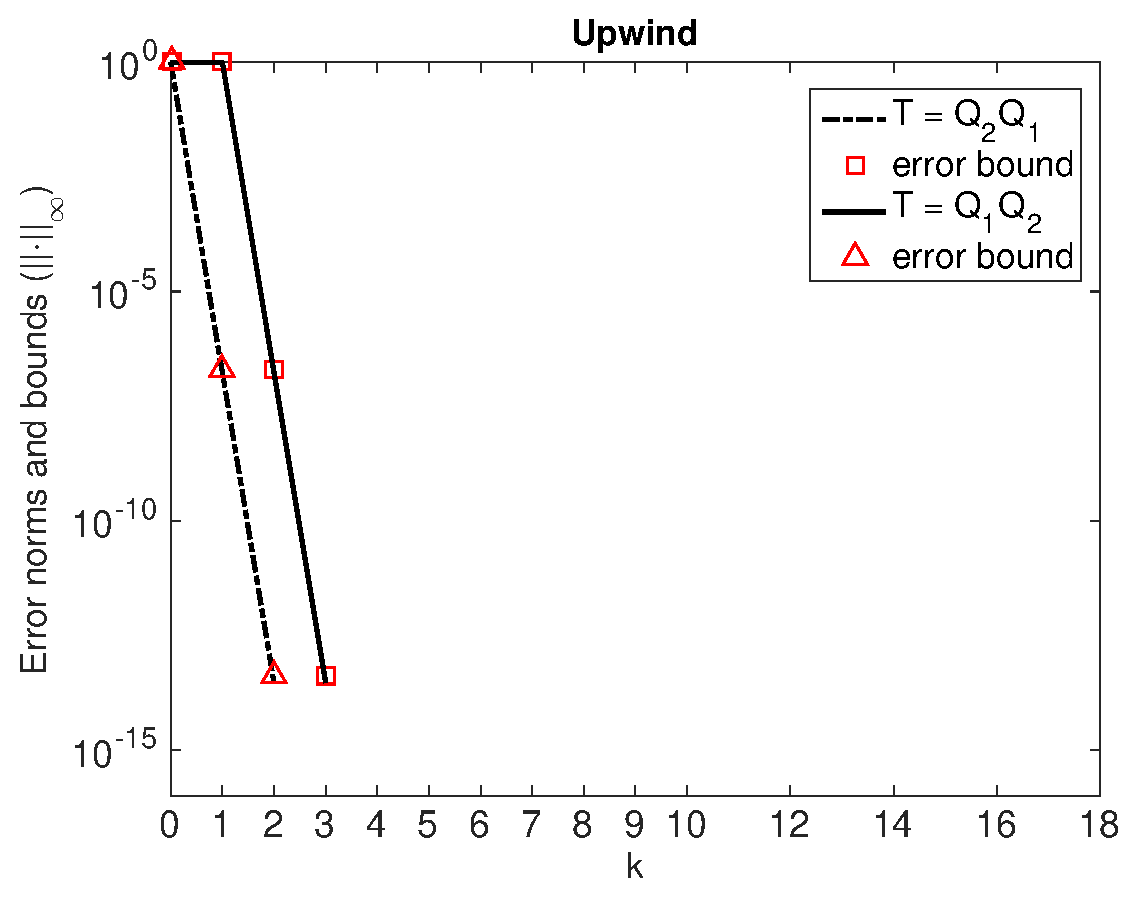
\includegraphics[width=0.95\linewidth]{figures/mSm_upwind2D_eps_1e-08_N_30_M_40}
\vspace*{-1em}
%\caption*{\footnotesize $\epsilon=10^{-4}$}\label{fig:err1_a}
\end{minipage}
%
\begin{minipage}[t]{0.5\linewidth}
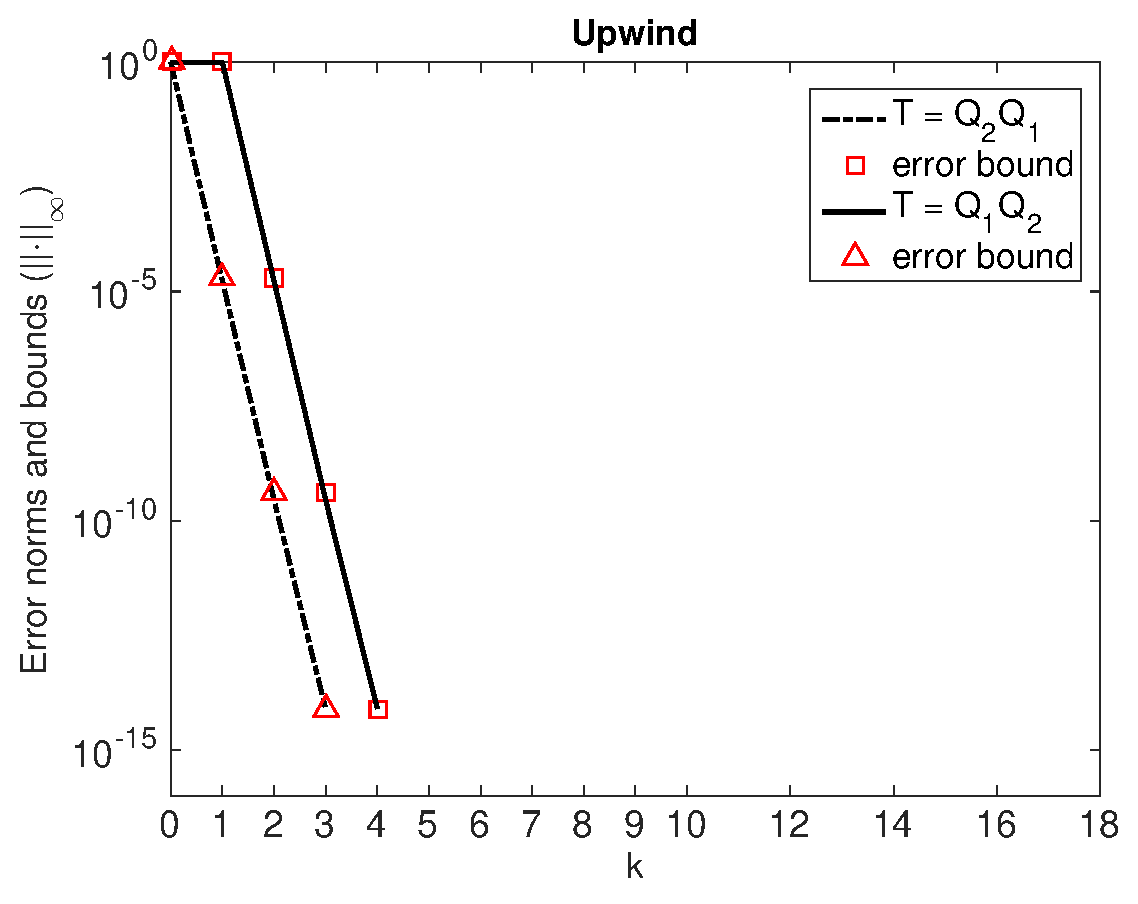
\includegraphics[width=0.95\linewidth]{figures/mSm_upwind2D_eps_1e-06_N_30_M_40}
\vspace*{-1em}
%\caption*{\footnotesize $\epsilon=10^{-8}$}\label{fig:err1_b}
\end{minipage}
\vspace*{-1em}
\caption{Convergence of multiplicative Schwarz and error bounds for $\epsilon=10^{-8}$ [l.], $\epsilon=10^{-6}$ [r.], and $\A \in \mathbb{R}^{1131\times1131}$.}\label{fig:2D:err1}
\end{figure}
%
\begin{figure}[tbhp]
\hspace*{-0.5em}
\begin{minipage}[t]{0.5\linewidth}
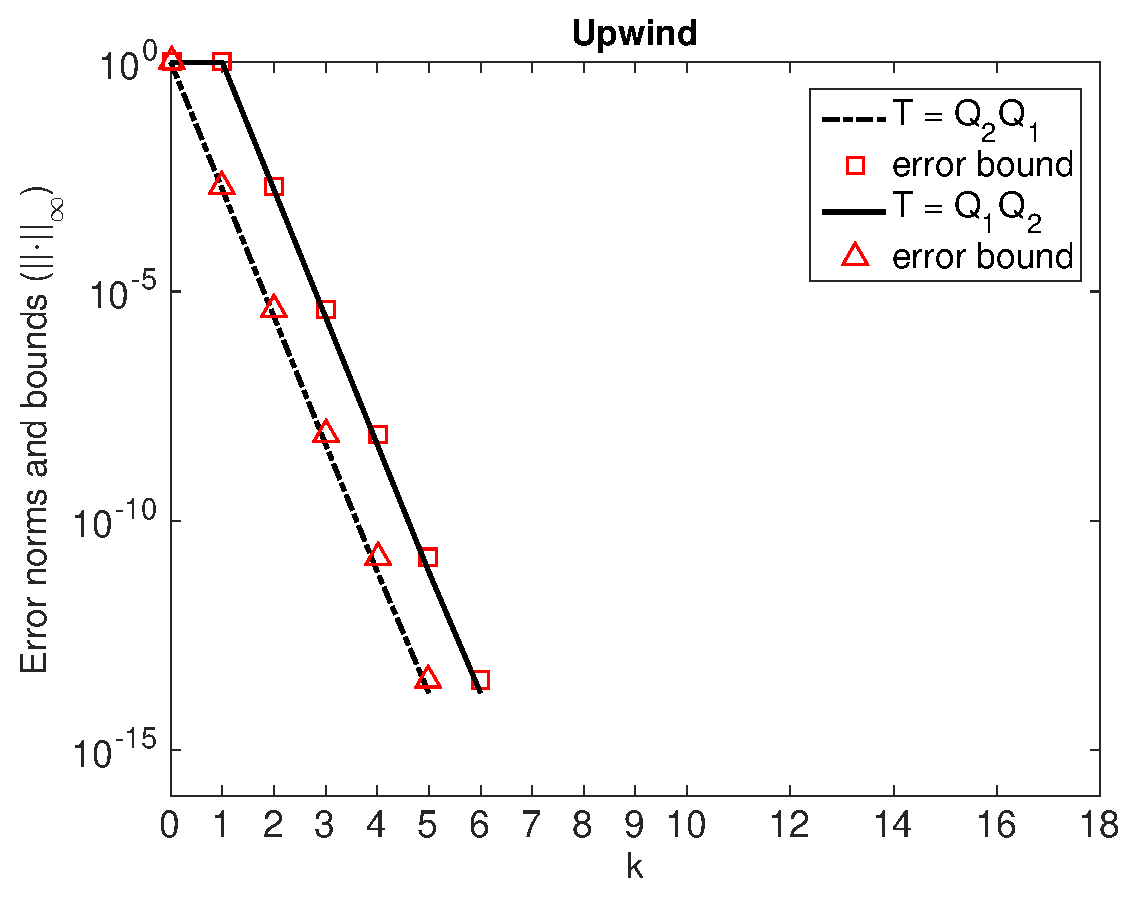
\includegraphics[width=0.95\linewidth]{figures/mSm_upwind2D_eps_1e-04_N_30_M_40}
\vspace*{-1em}
%\caption*{\footnotesize $\epsilon=10^{-4}$}\label{fig:err1_a}
\end{minipage}
%
\begin{minipage}[t]{0.5\linewidth}
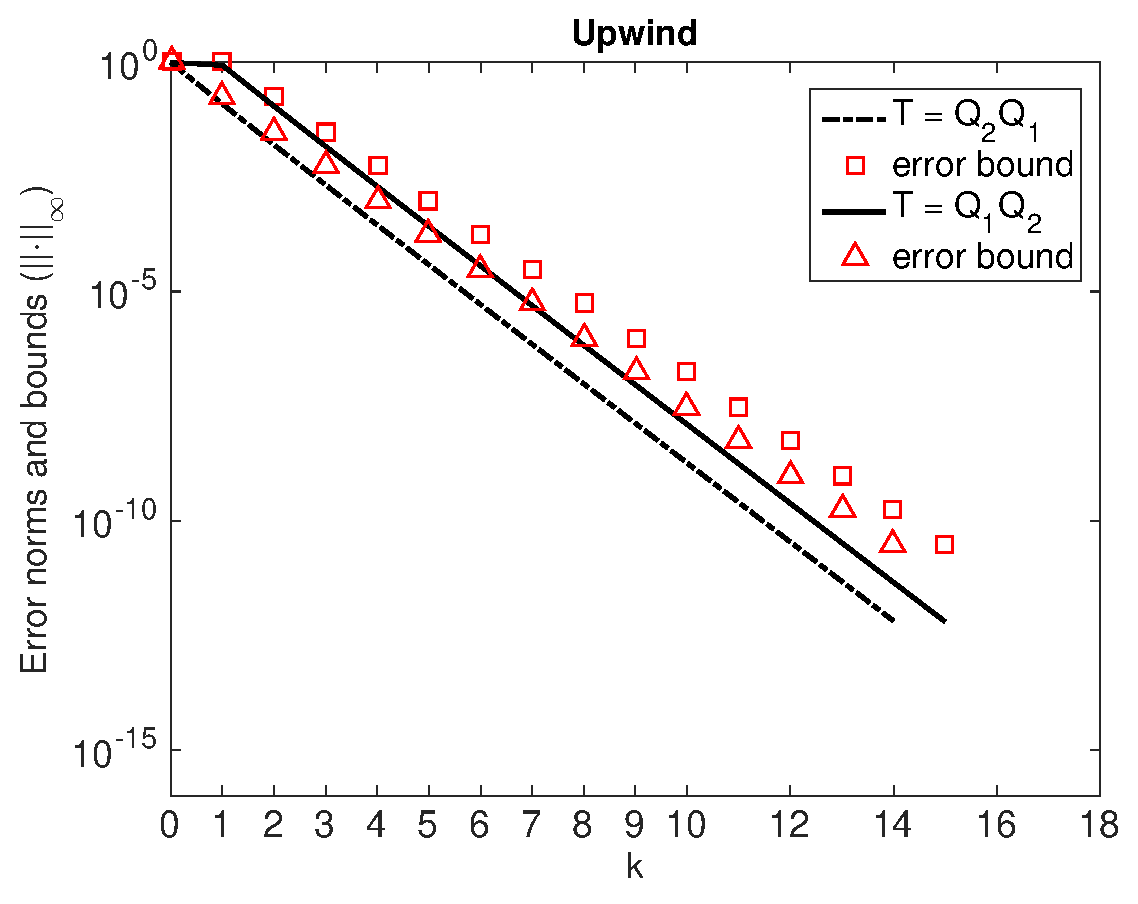
\includegraphics[width=0.95\linewidth]{figures/mSm_upwind2D_eps_1e-02_N_30_M_40}
\vspace*{-1em}
%\caption*{\footnotesize $\epsilon=10^{-8}$}\label{fig:err1_b}
\end{minipage}
\vspace*{-1em}
\caption{Convergence of multiplicative Schwarz and error bounds for $\epsilon=10^{-4}$ [l.], $\epsilon=10^{-2}$ [r.], and $\A \in \mathbb{R}^{1131\times1131}$.}\label{fig:2D:err2}
\end{figure}

We observe that the bounds are extremely close to the actual errors
produced by the method. Just like the bounds for the one-dimensional case, the
bounds for this two-dimensional case also predict the initial stagnation phase
of the multiplicative Schwarz method for the iteration matrix
$\T_{21}=\Q_1\Q_2$, making the bounds not only good quantitative measures for
the method's behavior but also provide a very good qualitative description of
it (see Table~\ref{tab:2D:rho}). Although the quality of the bounds decreases
as the problems become less convection dominated, the bounds given by
\eqref{eq:2D:T_bound_CD} and \eqref{eq:2D:T_bound_CD2} are still tight and
descriptive for perturbation parameters up to $\epsilon\leq10^{-2}$. We also
run the experiments for larger values of $N$ and $M$. The values of the
convergence factor $|\rho|$ as given in \eqref{eq:2D:rho} with
$\|\cdot\|=\|\cdot\|_{\infty}$ and the corresponding bound from
Corollary~\ref{cor:2D:conv-diff} are shown in
Table~\ref{tab:2D:rho} for different values of $\epsilon$.
%
% \begin{table}[tbhp]
% \centering
% %\begin{tabular}{rc|c||c|c}
% \begin{tabular}{r|c c}
%
% \cline{1-3}
% \multicolumn{3}{ c }{upwind}\\\hline
% %   & \multicolumn{2}{ c | }{upwind} & \multicolumn{2}{ c }{central differences}\\ \hline
% % \multicolumn{1}{ c|   }{$\epsilon$}&$|\rho|$~\eqref{eq:1D:rho} & bound~\eqref{eq:1D:bound_upw} & $|\rho|$~\eqref{eq:1D:rho} & bound~\eqref{eq:1D:bound2}\\
% %\hline
% \multicolumn{3}{c}{$N=M=9$, $\A\in\mathbb{R}^{81\times81}$}\\\hline
% %\multicolumn{1}{ c|  }{$10^{-9}$} & $2.9 \times 10^{-8}$ & $3.3 \times 10^{-8}$ & $1.8 \times 10^{-6}$ & $4.2 \times 10^{-6}$\\
% \multicolumn{1}{ c|   }{$\epsilon$}&$|\rho_{12}|$~\eqref{eq:2D:rho} & bound~\eqref{eq:2D:T_bound_CD}\\
% \multicolumn{1}{ c|  }{$10^{-8}$} & $3.1 \times 10^{-8}$ & $5.0 \times 10^{-8}$ \\
% \multicolumn{1}{ c|  }{$10^{-6}$} & $3.1 \times 10^{-6}$ & $5.0 \times 10^{-6}$ \\
% \multicolumn{1}{ c|  }{$10^{-4}$} & $3.1 \times 10^{-4}$ & $5.0 \times 10^{-4}$ \\
% \multicolumn{1}{ c|  }{$10^{-2}$} & $2.9 \times 10^{-2}$ & $5.5 \times 10^{-2}$ \\ \hline
% \multicolumn{3}{c}{$N=M=17$, $\A\in\mathbb{R}^{289\times289}$}\\\hline
% %\multicolumn{1}{ c|  }{$10^{-9}$} & $6.0 \times 10^{-8}$ & $6.5 \times 10^{-8}$ & $7.7 \times 10^{-6}$ & $1.7 \times 10^{-5}$\\
% \multicolumn{1}{ c|  }{$10^{-8}$} & $6.6 \times 10^{-8}$ & $9.0 \times 10^{-8}$ \\
% \multicolumn{1}{ c|  }{$10^{-6}$} & $6.6 \times 10^{-6}$ & $9.0 \times 10^{-6}$ \\
% \multicolumn{1}{ c|  }{$10^{-4}$} & $6.6 \times 10^{-4}$ & $9.0 \times 10^{-4}$ \\
% \multicolumn{1}{ c|  }{$10^{-2}$} & $6.1 \times 10^{-2}$ & $1.1 \times 10^{-1}$ \\ \hline
% \multicolumn{3}{c}{$N=M=33$, $\A\in\mathbb{R}^{1089\times1089}$}\\\hline
% %\multicolumn{1}{ c|  }{$10^{-9}$} & $1.2 \times 10^{-7}$ & $1.3 \times 10^{-7}$ & $3.2 \times 10^{-5}$ & $6.6 \times 10^{-5}$\\
% \multicolumn{1}{ c|  }{$10^{-8}$} & $1.4 \times 10^{-7}$ & $1.7 \times 10^{-7}$ \\
% \multicolumn{1}{ c|  }{$10^{-6}$} & $1.4 \times 10^{-5}$ & $1.7 \times 10^{-5}$ \\
% \multicolumn{1}{ c|  }{$10^{-4}$} & $1.4 \times 10^{-3}$ & $1.7 \times 10^{-3}$ \\
% \multicolumn{1}{ c|  }{$10^{-2}$} & $1.2 \times 10^{-1}$ & $2.2 \times 10^{-1}$ \\ \hline
% \multicolumn{3}{c}{$N=M=65$, $\A\in\mathbb{R}^{4225\times4225}$}\\\hline
% %\multicolumn{1}{ c|  }{$10^{-9}$} & $2.5 \times 10^{-7}$ & $2.6 \times 10^{-7}$ & $1.3 \times 10^{-4}$ & $2.6 \times 10^{-4}$\\
% \multicolumn{1}{ c|  }{$10^{-8}$} & $2.9 \times 10^{-7}$ & $3.3 \times 10^{-7}$ \\
% \multicolumn{1}{ c|  }{$10^{-6}$} & $2.9 \times 10^{-5}$ & $3.3 \times 10^{-5}$ \\
% \multicolumn{1}{ c|  }{$10^{-4}$} & $2.9 \times 10^{-3}$ & $3.3 \times 10^{-3}$ \\
% \multicolumn{1}{ c|  }{$10^{-2}$} & $2.2 \times 10^{-1}$ & $5.6 \times 10^{-1}$ \\ \hline
% % \multicolumn{3}{c}{$N=M=129$, $\A\in\mathbb{R}^{16641\times16641}$}\\\hline
% % %\multicolumn{1}{ c|  }{$10^{-9}$} & $5.1 \times 10^{-7}$ & $5.1 \times 10^{-7}$ & $5.2 \times 10^{-4}$ & $1.1 \times 10^{-3}$\\
% % \multicolumn{1}{ c|  }{$10^{-8}$} & $5.1 \times 10^{-6}$ & $5.1 \times 10^{-6}$ \\
% % \multicolumn{1}{ c|  }{$10^{-6}$} & $5.1 \times 10^{-4}$ & $5.1 \times 10^{-4}$ \\
% % \multicolumn{1}{ c|  }{$10^{-4}$} & $4.8 \times 10^{-2}$ & $4.9 \times 10^{-2}$ \\
% % \multicolumn{1}{ c|  }{$10^{-2}$} & $8.4 \times 10^{-1}$ & $8.6 \times 10^{-1}$ \\ \hline
% % \multicolumn{3}{c}{$N=2050$}\\\hline
% % %\multicolumn{1}{ c|  }{$10^{-9}$} & $1.0 \times 10^{-6}$ & $1.0 \times 10^{-6}$ & $2.1 \times 10^{-3}$ & $4.2 \times 10^{-3}$\\
% % \multicolumn{1}{ c|  }{$10^{-8}$} & $1.0 \times 10^{-5}$ & $1.0 \times 10^{-5}$ \\
% % \multicolumn{1}{ c|  }{$10^{-6}$} & $1.0 \times 10^{-3}$ & $1.0 \times 10^{-3}$ \\
% % \multicolumn{1}{ c|  }{$10^{-4}$} & $9.2 \times 10^{-2}$ & $9.3 \times 10^{-2}$ \\
% % \multicolumn{1}{ c|  }{$10^{-2}$} & $9.1 \times 10^{-1}$ & $9.2 \times 10^{-1}$ \\ \hline
% % \multicolumn{3}{c}{$N=4098$}\\\hline
% % %\multicolumn{1}{ c|  }{$10^{-9}$} & $2.0 \times 10^{-6}$ & $2.0 \times 10^{-6}$ & $8.4 \times 10^{-3}$ & $1.7 \times 10^{-2}$\\
% % \multicolumn{1}{ c|  }{$10^{-8}$} & $2.0 \times 10^{-5}$ & $2.0 \times 10^{-5}$ \\
% % \multicolumn{1}{ c|  }{$10^{-6}$} & $2.0 \times 10^{-3}$ & $2.0 \times 10^{-3}$ \\
% % \multicolumn{1}{ c|  }{$10^{-4}$} & $1.7 \times 10^{-1}$ & $1.7 \times 10^{-1}$ \\
% % \multicolumn{1}{ c|  }{$10^{-2}$} & $9.5 \times 10^{-1}$ & $9.6 \times 10^{-1}$ \\ \hline
% % \multicolumn{3}{c}{$N=8194$}\\\hline
% % \multicolumn{1}{ c|  }{$10^{-8}$} & $4.1 \times 10^{-5}$ & $4.1 \times 10^{-5}$ \\
% % \multicolumn{1}{ c|  }{$10^{-6}$} & $4.1 \times 10^{-3}$ & $4.1 \times 10^{-3}$ \\
% % \multicolumn{1}{ c|  }{$10^{-4}$} & $2.9 \times 10^{-1}$ & $2.9 \times 10^{-1}$ \\
% % \multicolumn{1}{ c|  }{$10^{-2}$} & $9.8 \times 10^{-1}$ & $9.8 \times 10^{-1}$ \\
% % & \multicolumn{2}{ c | }{upwind} & \multicolumn{2}{ c }{central differences}\\
% %\hline
% \multicolumn{1}{ c|   }{$\epsilon$}&$|\rho_{12}|$~\eqref{eq:2D:rho} & bound~\eqref{eq:2D:T_bound_CD}\\ \hline
% \end{tabular}
% \caption{Values of $|\rho_{12}|$ computed using \eqref{eq:2D:rho} and the corresponding bound \eqref{eq:2D:T_bound_CD} for different values of $N$, $M$ and $\epsilon$.}
% \label{tab:2D:rho}
% \end{table}



\begin{table}[tbhp]
\hspace*{2em}
\begin{minipage}[t]{0.5\linewidth}
\begin{tabular}{r|c c}
\cline{1-3}
\multicolumn{3}{c}{$N=20,M=20$, $\A\in\mathbb{R}^{361\times361}$}\\\hline
\multicolumn{1}{ c|   }{$\epsilon$}& $\rho_{12}$ in~\eqref{eq:2D:rho} &
$\rho$ in~\eqref{eq:2D:T_bound_CD2}\\
\multicolumn{1}{ c|  }{$10^{-8}$} & $7.5 \times 10^{-8}$ & $1.0 \times 10^{-7}$ \\
\multicolumn{1}{ c|  }{$10^{-6}$} & $7.5 \times 10^{-6}$ & $1.0 \times 10^{-5}$ \\
\multicolumn{1}{ c|  }{$10^{-4}$} & $7.5 \times 10^{-4}$ & $1.0 \times 10^{-3}$ \\
\multicolumn{1}{ c|  }{$10^{-2}$} & $7.0 \times 10^{-2}$ & $9.6 \times 10^{-2}$ \\ \hline
\multicolumn{3}{c}{$N=30, M=30$, $\A\in\mathbb{R}^{841\times841}$}\\\hline
\multicolumn{1}{ c|  }{$10^{-8}$} & $1.2 \times 10^{-7}$ & $1.5 \times 10^{-7}$ \\
\multicolumn{1}{ c|  }{$10^{-6}$} & $1.2 \times 10^{-5}$ & $1.5 \times 10^{-5}$ \\
\multicolumn{1}{ c|  }{$10^{-4}$} & $1.2 \times 10^{-3}$ & $1.5 \times 10^{-3}$ \\
\multicolumn{1}{ c|  }{$10^{-2}$} & $1.1 \times 10^{-1}$ & $1.4 \times 10^{-1}$ \\ \hline
\multicolumn{3}{c}{$N=40,M=40$, $\A\in\mathbb{R}^{1521\times1521}$}\\\hline
\multicolumn{1}{ c|  }{$10^{-8}$} & $1.7 \times 10^{-7}$ & $2.0 \times 10^{-7}$ \\
\multicolumn{1}{ c|  }{$10^{-6}$} & $1.7 \times 10^{-5}$ & $2.0 \times 10^{-5}$ \\
\multicolumn{1}{ c|  }{$10^{-4}$} & $1.7 \times 10^{-3}$ & $2.0 \times 10^{-3}$ \\
\multicolumn{1}{ c|  }{$10^{-2}$} & $1.4 \times 10^{-1}$ & $1.8 \times 10^{-1}$ \\\hline
\multicolumn{3}{c}{$N=50,M=50$, $A\in\mathbb{R}^{2401\times2401}$}\\\hline
\multicolumn{1}{ c|  }{$10^{-8}$} & $2.2 \times 10^{-7}$ & $2.5 \times 10^{-7}$ \\
\multicolumn{1}{ c|  }{$10^{-6}$} & $2.2 \times 10^{-5}$ & $2.5 \times 10^{-5}$ \\
\multicolumn{1}{ c|  }{$10^{-4}$} & $2.2 \times 10^{-3}$ & $2.5 \times 10^{-3}$ \\
\multicolumn{1}{ c|  }{$10^{-2}$} & $1.8 \times 10^{-1}$ & $2.1 \times 10^{-1}$ \\
\end{tabular}
\end{minipage}
%
\begin{minipage}[t]{0.5\linewidth}
\begin{tabular}{r|c c}
\cline{1-3}
\multicolumn{3}{c}{$N=20, M=30$, $\A\in\mathbb{R}^{551\times551}$}\\\hline
\multicolumn{1}{ c|   }{$\epsilon$}& $\rho_{12}$ in~\eqref{eq:2D:rho} &
$\rho$ in~\eqref{eq:2D:T_bound_CD2}\\
\multicolumn{1}{ c|  }{$10^{-8}$} & $1.2 \times 10^{-7}$ & $1.5 \times 10^{-7}$ \\
\multicolumn{1}{ c|  }{$10^{-6}$} & $1.2 \times 10^{-5}$ & $1.5 \times 10^{-5}$ \\
\multicolumn{1}{ c|  }{$10^{-4}$} & $1.2 \times 10^{-3}$ & $1.5 \times 10^{-3}$ \\
\multicolumn{1}{ c|  }{$10^{-2}$} & $1.1 \times 10^{-1}$ & $1.4 \times 10^{-1}$ \\ \hline
\multicolumn{3}{c}{$N=30,M=40$, $\A\in\mathbb{R}^{1131\times1131}$}\\\hline
\multicolumn{1}{ c|  }{$10^{-8}$} & $1.7 \times 10^{-7}$ & $2.0 \times 10^{-7}$ \\
\multicolumn{1}{ c|  }{$10^{-6}$} & $1.7 \times 10^{-5}$ & $2.0 \times 10^{-5}$ \\
\multicolumn{1}{ c|  }{$10^{-4}$} & $1.7 \times 10^{-3}$ & $2.0 \times 10^{-3}$ \\
\multicolumn{1}{ c|  }{$10^{-2}$} & $1.4 \times 10^{-1}$ & $1.8 \times 10^{-1}$ \\\hline
\multicolumn{3}{c}{$N=40, M=50$, $\A\in\mathbb{R}^{1911\times1911}$}\\\hline
\multicolumn{1}{ c|  }{$10^{-8}$} & $2.2 \times 10^{-7}$ & $2.5 \times 10^{-7}$ \\
\multicolumn{1}{ c|  }{$10^{-6}$} & $2.2 \times 10^{-5}$ & $2.5 \times 10^{-5}$ \\
\multicolumn{1}{ c|  }{$10^{-4}$} & $2.2 \times 10^{-3}$ & $2.5 \times 10^{-3}$ \\
\multicolumn{1}{ c|  }{$10^{-2}$} & $1.8 \times 10^{-1}$ & $2.1 \times 10^{-1}$ \\ \hline
\multicolumn{3}{c}{$N=50,M=60$, $\A\in\mathbb{R}^{2891\times2891}$}\\\hline
\multicolumn{1}{ c|  }{$10^{-8}$} & $2.6 \times 10^{-7}$ & $3.0 \times 10^{-7}$ \\
\multicolumn{1}{ c|  }{$10^{-6}$} & $2.6 \times 10^{-5}$ & $3.0 \times 10^{-5}$ \\
\multicolumn{1}{ c|  }{$10^{-4}$} & $2.6 \times 10^{-3}$ & $3.0 \times 10^{-3}$ \\
\multicolumn{1}{ c|  }{$10^{-2}$} & $2.1 \times 10^{-1}$ & $2.5 \times 10^{-1}$ \\
\end{tabular}
\end{minipage}\\[1ex]
\caption{Values of $|\rho_{12}|$ computed using \eqref{eq:2D:rho} with
$\|\cdot\|=\|\cdot\|_{\infty}$ and the corresponding bound \eqref{eq:2D:T_bound_CD2} for different values of $N$, $M$ and $\epsilon$.}
\label{tab:2D:rho}
\end{table}

We continue our numerical experiments  by applying GMRES to the linear
algebraic system \emph{preconditioned with multiplicative Schwarz}, i.e., the
linear algebraic system \eqref{eq:2D:precond}, in the case $N=30$ and $M=40$.
On the right side of Figures~\ref{fig:2D:prec1}--\ref{fig:2D:prec4} the
preconditioned relative residual norms are shown for a specific value of
$\epsilon$ and incresing values of the iteration step $k$. Convergence within a
tolerance of $10^{-14}$ is always achieved in less than $N$ iterations for the
preconditioned systems, sometimes reaching the tolerance in only 2 iterations.
This is a dramatic improvement compared to the behavior of the unpreconditioned
GMRES method (shown in the left side of each figure) which does not converge to
the same tolerance in less than 320 iterations for the chosen set of parameters.
%
\begin{figure}[tbhp]
\hspace*{-0.5em}
\begin{minipage}[t]{0.5\linewidth}
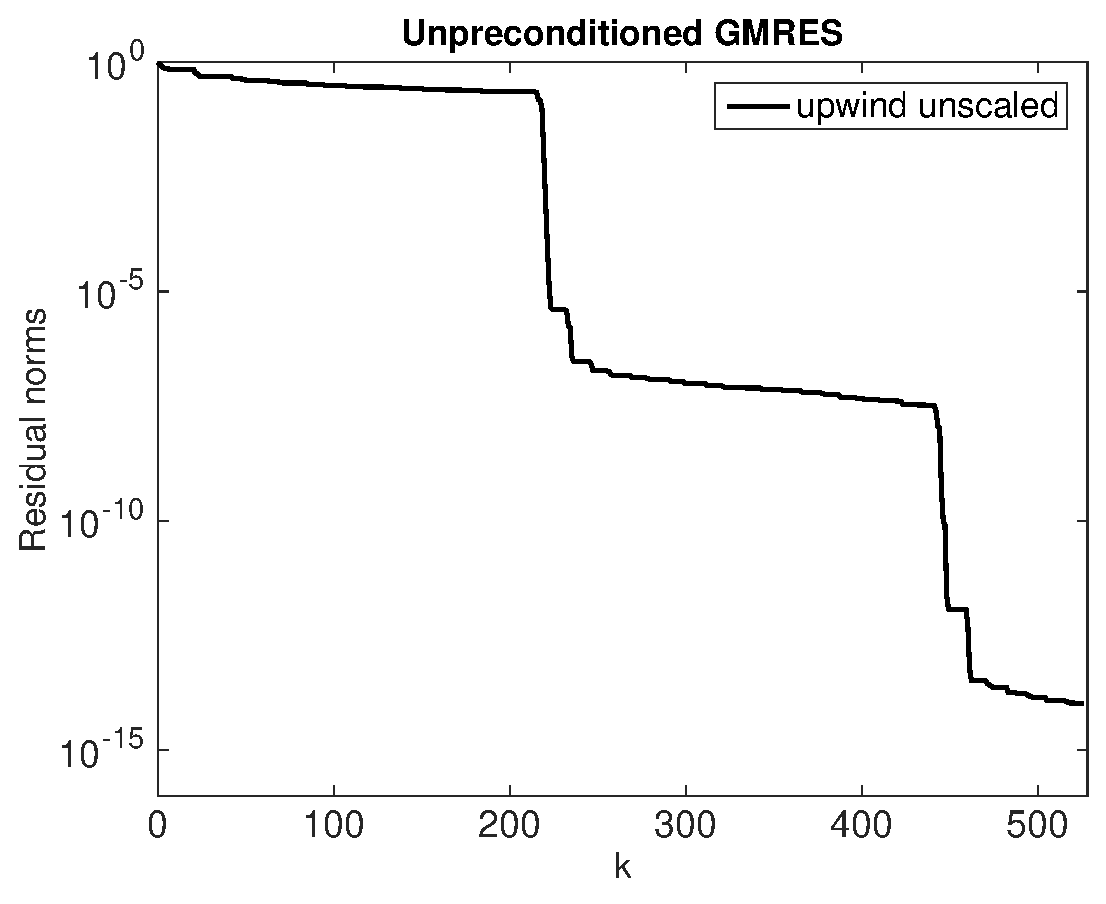
\includegraphics[width=0.95\linewidth]{figures/gmres_upwind2D_eps_1e-08_N_30_M_40}
\vspace*{-1em}
%\caption*{\footnotesize $\epsilon=10^{-4}$}\label{fig:err1_a}
\end{minipage}
%
\begin{minipage}[t]{0.5\linewidth}
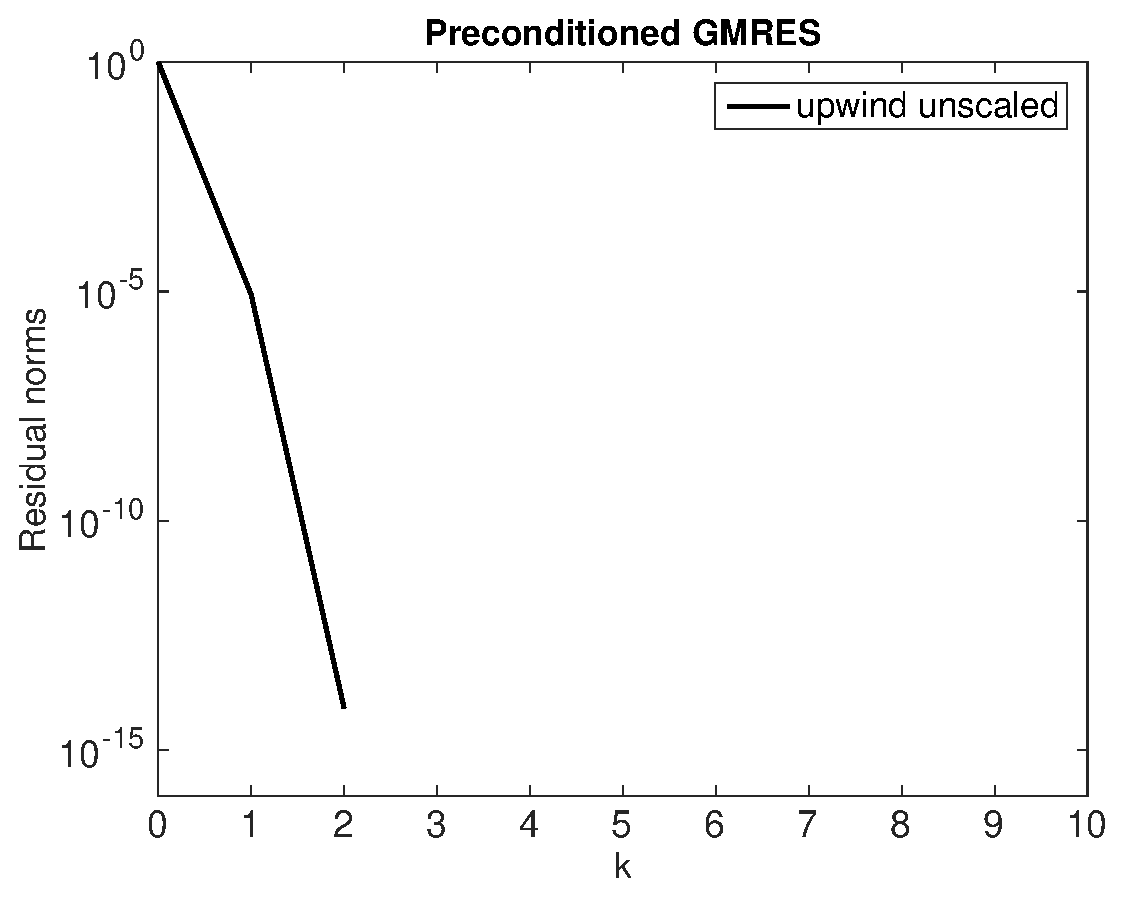
\includegraphics[width=0.95\linewidth]{figures/gmres_precond_upwind2D_eps_1e-06_N_30_M_40}
\vspace*{-1em}
%\caption*{\footnotesize $\epsilon=10^{-8}$}\label{fig:err1_b}
\end{minipage}
\vspace*{-1em}
\caption{Unpreconditioned [l.] and preconditioned [r.] GMRES convergence for $\epsilon=10^{-8}$ and $\A \in \mathbb{R}^{1131\times1131}$.}\label{fig:2D:prec1}
\end{figure}
%
\begin{figure}[tbhp]
\hspace*{-0.5em}
\begin{minipage}[t]{0.5\linewidth}
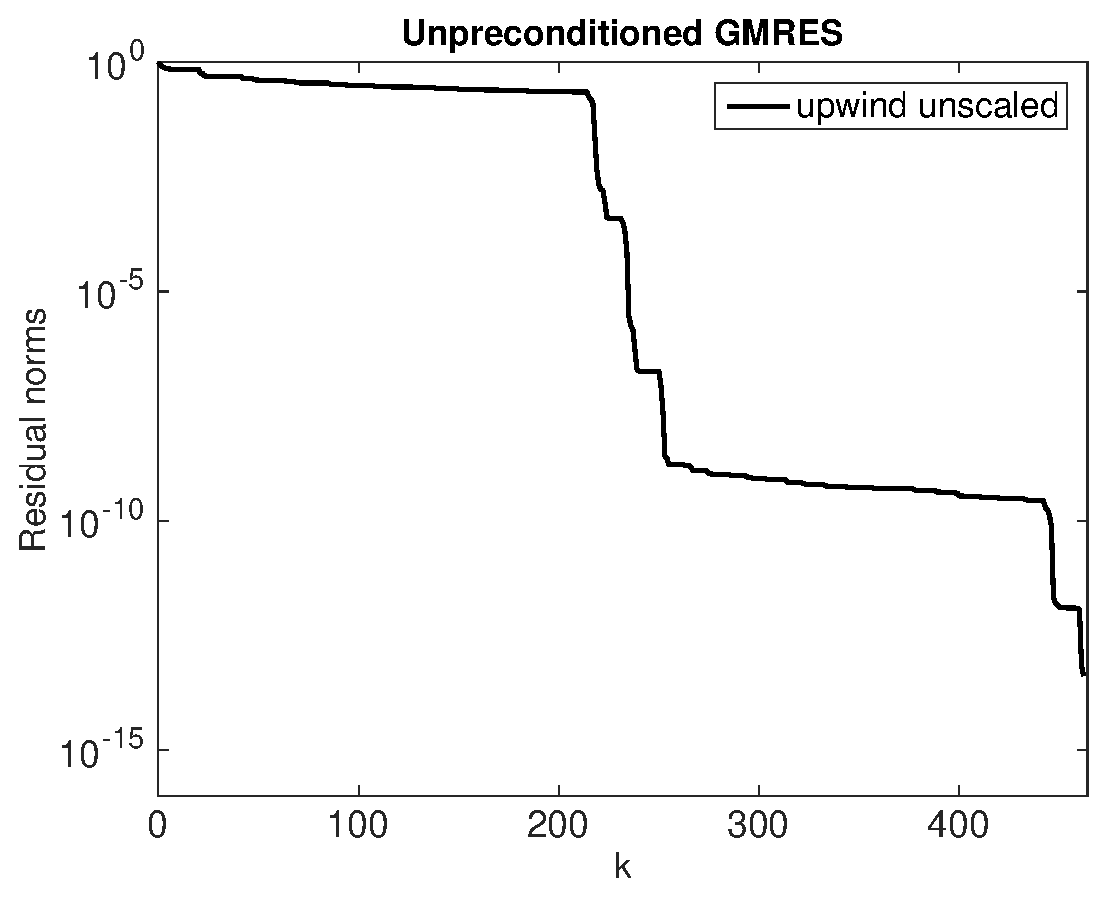
\includegraphics[width=0.95\linewidth]{figures/gmres_upwind2D_eps_1e-06_N_30_M_40}
\vspace*{-1em}
%\caption*{\footnotesize $\epsilon=10^{-4}$}\label{fig:err1_a}
\end{minipage}
%
\begin{minipage}[t]{0.5\linewidth}
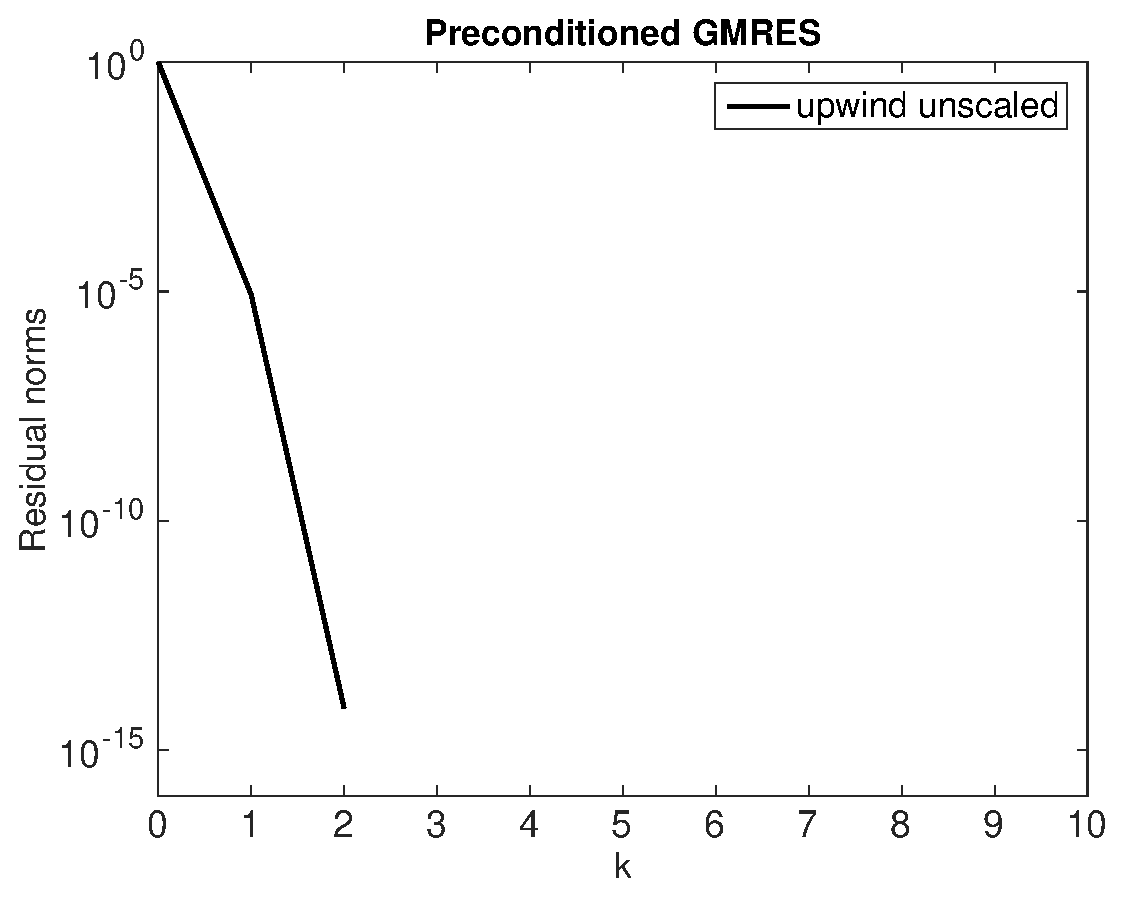
\includegraphics[width=0.95\linewidth]{figures/gmres_precond_upwind2D_eps_1e-06_N_30_M_40}
\vspace*{-1em}
%\caption*{\footnotesize $\epsilon=10^{-8}$}\label{fig:err1_b}
\end{minipage}
\vspace*{-1em}
\caption{Unpreconditioned [l.] and preconditioned [r.] GMRES convergence for $\epsilon=10^{-6}$ and $\A \in \mathbb{R}^{1131\times1131}$.}\label{fig:2D:prec2}
\end{figure}
%
\begin{figure}[tbhp]
\hspace*{-0.5em}
\begin{minipage}[t]{0.5\linewidth}
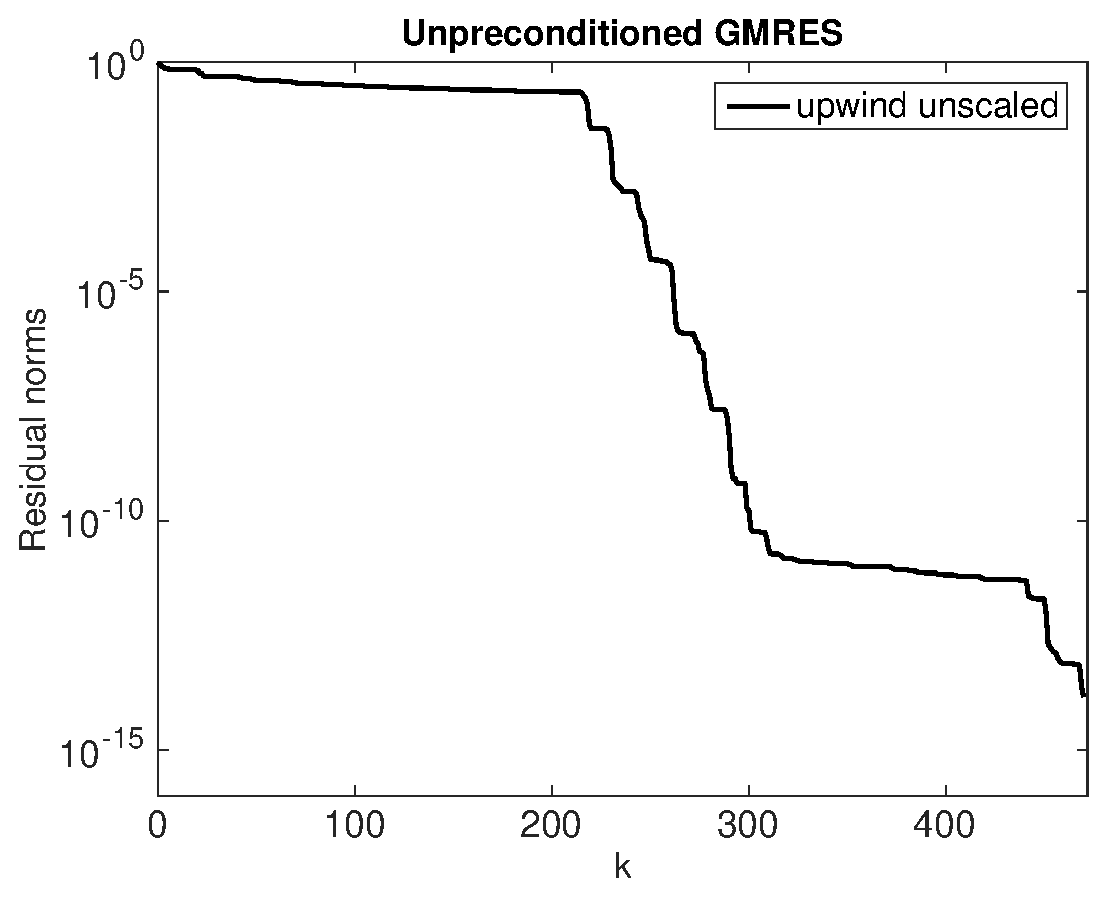
\includegraphics[width=0.95\linewidth]{figures/gmres_upwind2D_eps_1e-04_N_30_M_40}
\vspace*{-1em}
%\caption*{\footnotesize $\epsilon=10^{-4}$}\label{fig:err1_a}
\end{minipage}
\vspace*{-1em}
\begin{minipage}[t]{0.5\linewidth}
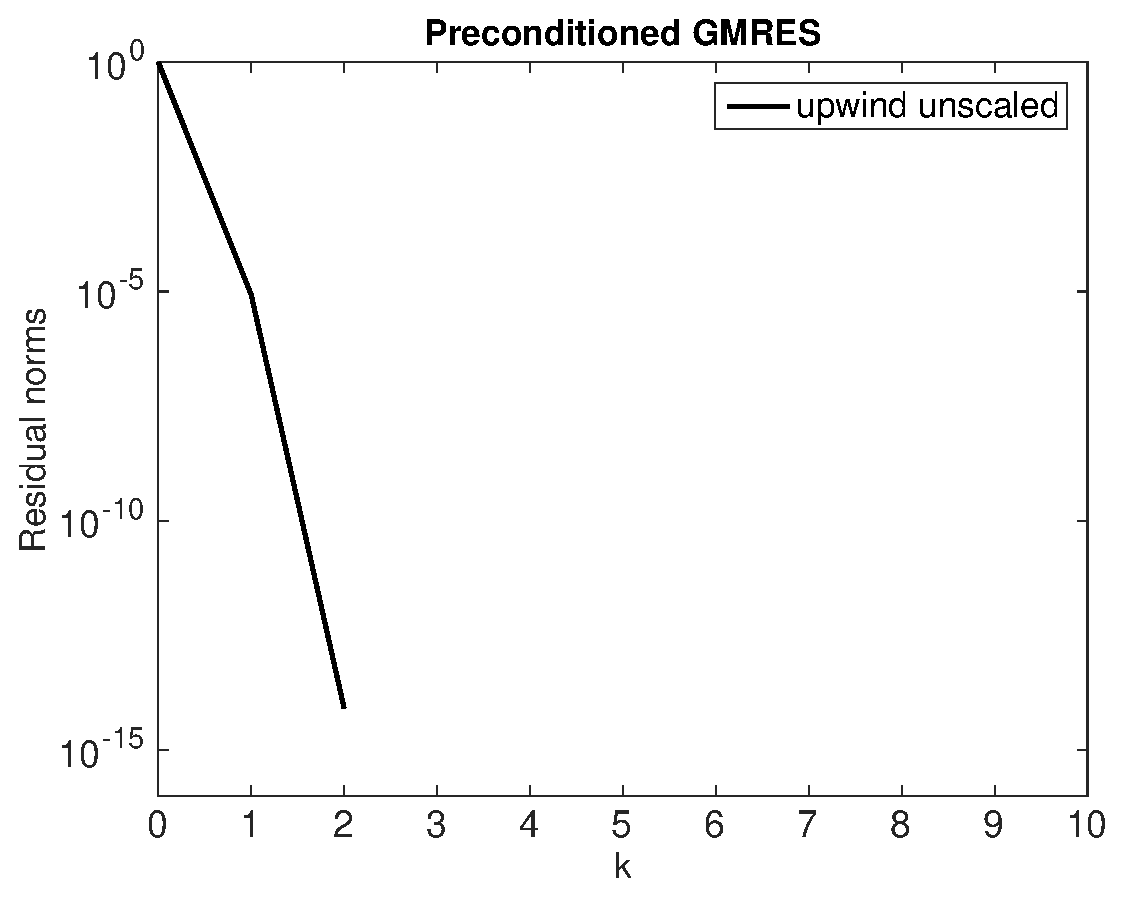
\includegraphics[width=0.95\linewidth]{figures/gmres_precond_upwind2D_eps_1e-06_N_30_M_40}
\vspace*{-1em}
%\caption*{\footnotesize $\epsilon=10^{-8}$}\label{fig:err1_b}
\end{minipage}
\vspace*{-1em}
\caption{Unpreconditioned [l.] and preconditioned [r.] GMRES convergence for $\epsilon=10^{-4}$ and $\A \in \mathbb{R}^{1131\times1131}$.}\label{fig:2D:prec3}
\end{figure}
%
\begin{figure}[tbhp]
\hspace*{-0.5em}
\begin{minipage}[t]{0.5\linewidth}
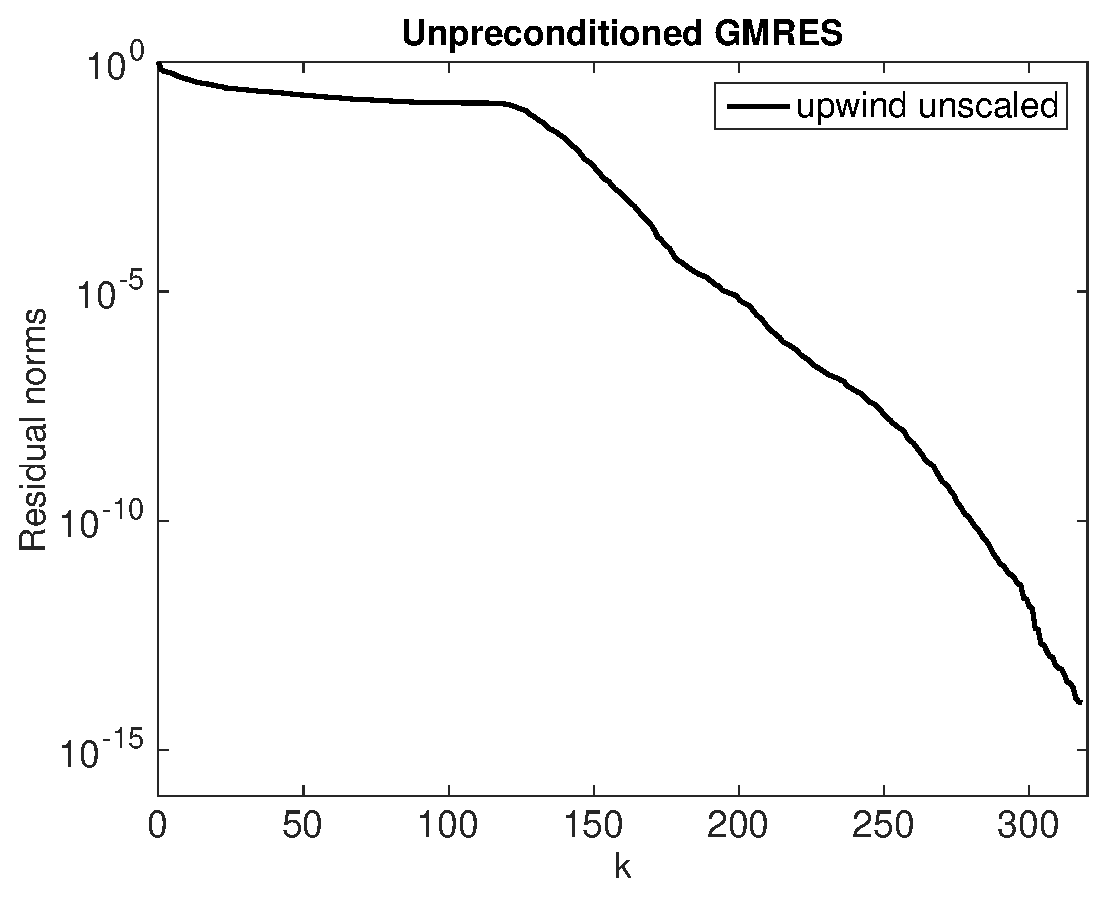
\includegraphics[width=0.95\linewidth]{figures/gmres_upwind2D_eps_1e-02_N_30_M_40}
\vspace*{-1em}
%\caption*{\footnotesize $\epsilon=10^{-4}$}\label{fig:err1_a}
\end{minipage}
%
\begin{minipage}[t]{0.5\linewidth}
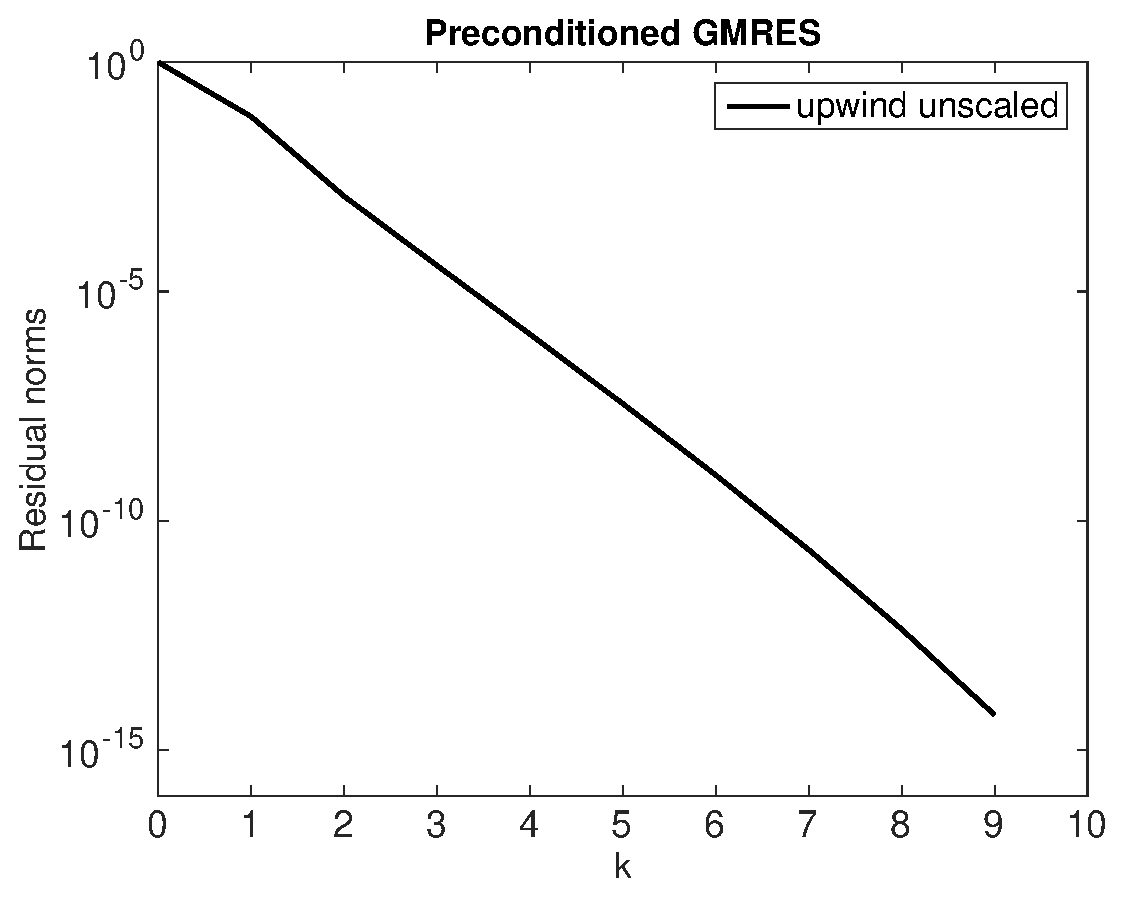
\includegraphics[width=0.95\linewidth]{figures/gmres_precond_upwind2D_eps_1e-02_N_30_M_40}
\vspace*{-1em}
%\caption*{\footnotesize $\epsilon=10^{-8}$}\label{fig:err1_b}
\end{minipage}
\vspace*{-1em}
\caption{Unpreconditioned [l.] and preconditioned [r.] GMRES convergence for $\epsilon=10^{-2}$ and $\A \in \mathbb{R}^{1131\times1131}$.}\label{fig:2D:prec4}
\end{figure}
%

\pagebreak
In the numerical experiments presented so far, the local subdomain problems
\eqref{eq:2D:localsub} were assumed to be solved exactly, since the inverses of
the matrices $\A_i$ were calculated using the backslash operator in
\texttt{MATLAB}. Nevertheless, as we have discussed previously (see
Sections~\ref{2D:precon} and \ref{1D:ShishScwarzPrecon}), very often in
practice the solutions to linear systems with the matrices $\A_i$ are only
solved approximately. We conclude our numerical experiments by
presenting results for the preconditioned GMRES method for the case of inexact
local solves.
% For the case of $N=30$, $M=40$ and $\epsilon=10^{-8}$
% Figures~\ref{fig:2D:GMRES.inexact.prec.N30.M40.eps8.tol1_2}--\ref{fig:2D:GMRES.inexact.prec.N30.M40.eps8.tol3_4}
% show the preconditioned relative residual norms for the case where the local
% solves are performed using the GMRES method (dotted line) as well as the
% residual norms for the case where they are solved exactly (using
% \texttt{MATLAB}'s backslash operator) for comparison (solid line).
% For this specific value of the perturbation parameter, the figures show that by choosing a tolerance of $10^{-2}$ for the residual minimization accuracy in the solution of the local subdomain problems, the number of steps needed for the convergence of GMRES to reach a normwise relative residual of $10^{-14}$ in the global system (outer iteration) for the upwind scheme grows from 2 to 5 steps only. In contrast to the results for the one-dimensional problem, increasing the
% accuracy of solution of the local subdomain problems does not improve the
% number of iterations needed for the outer iteration of GMRES to reach the same
% solution, i.e. by solving the local subdomain problems inexactly (and therefore
% reducing the most computationally intensive part of this solution approach) our
% approach leads to a very fast preconditioning method.
%
%
% \begin{figure}[tbhp]
% \begin{minipage}[t]{0.48\linewidth}
% 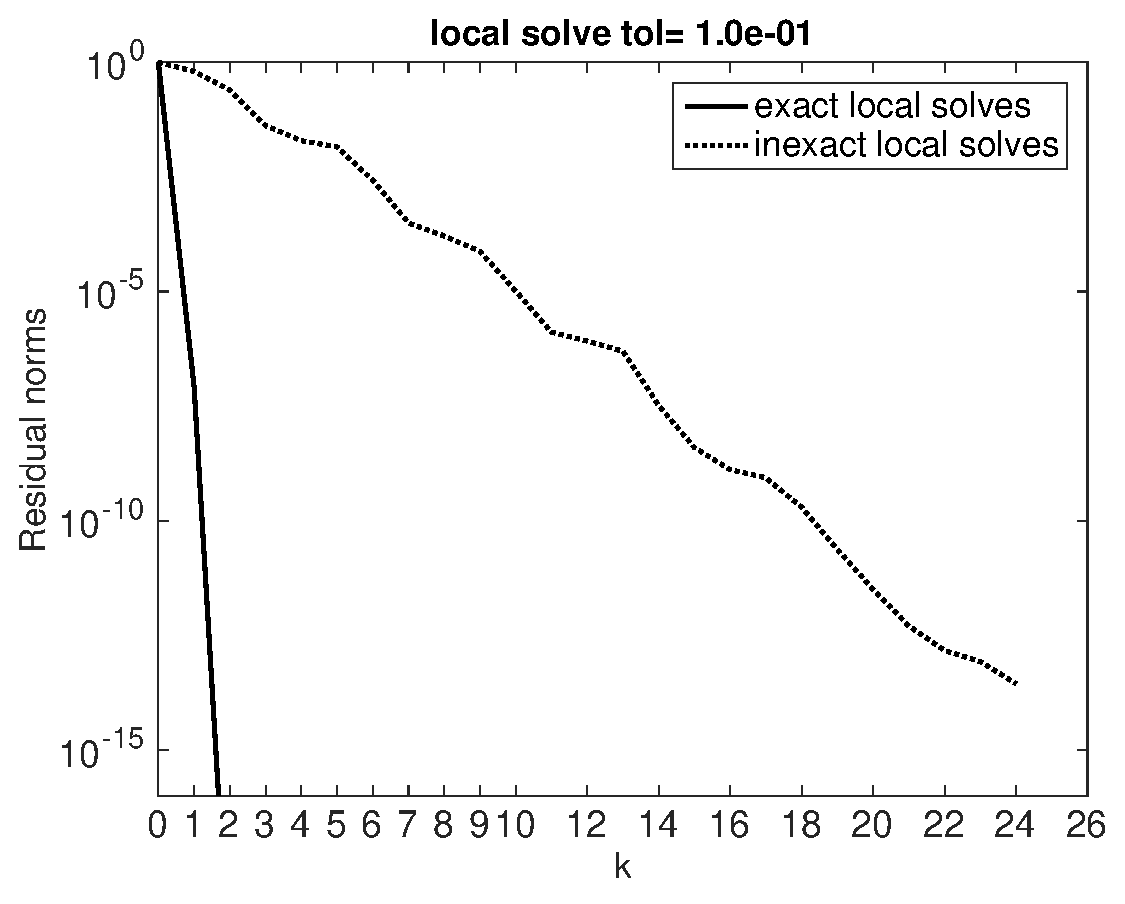
\includegraphics[width=0.98\linewidth]{figures/gmres_precond_upwind2D_eps_1e-08_inexact-1e-01_N_30_M_40}
% %\label{fig:1D:GMRES.N198.eps4.prec}
% % note: if changing to 3 figures again, it needs to be changed in two places
% %\caption{Preconditioned GMRES convergence for $\epsilon=10^{-4}$.}
% \end{minipage}
% %
% \begin{minipage}[t]{0.48\linewidth}
% 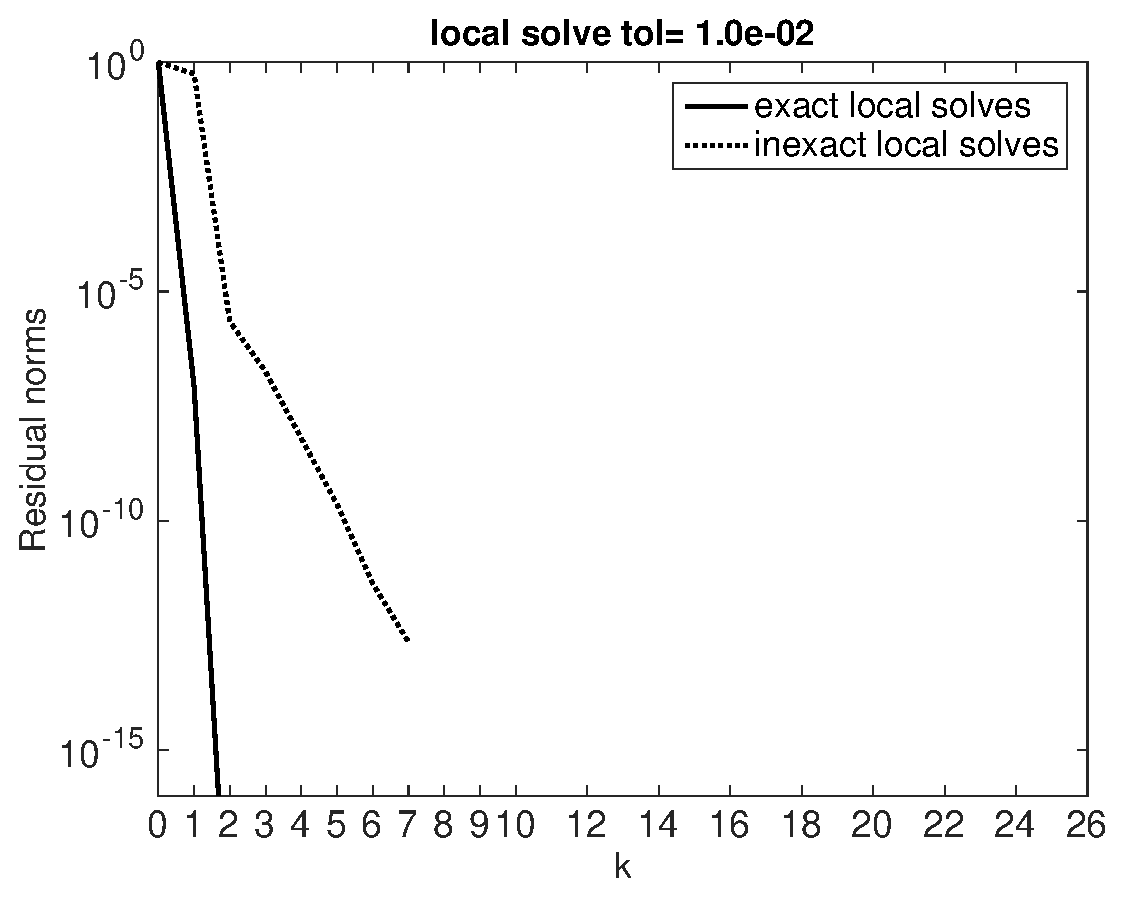
\includegraphics[width=0.98\linewidth]{figures/gmres_precond_upwind2D_eps_1e-08_inexact-1e-02_N_30_M_40}
% \end{minipage}
% \caption{Unpreconditioned and preconditioned GMRES convergence for $\epsilon~=~10^{-8}$ with inexact localsolve tolerance of $10^{-1}$ [l.] and $10^{-2}$ [r.].}
% \label{fig:2D:GMRES.inexact.prec.N30.M40.eps8.tol1_2}
% \end{figure}
% %
% \begin{figure}[tbhp]
% \hspace{-1cm}
% \centering
% \begin{minipage}[t]{0.48\linewidth}
% \centering
% 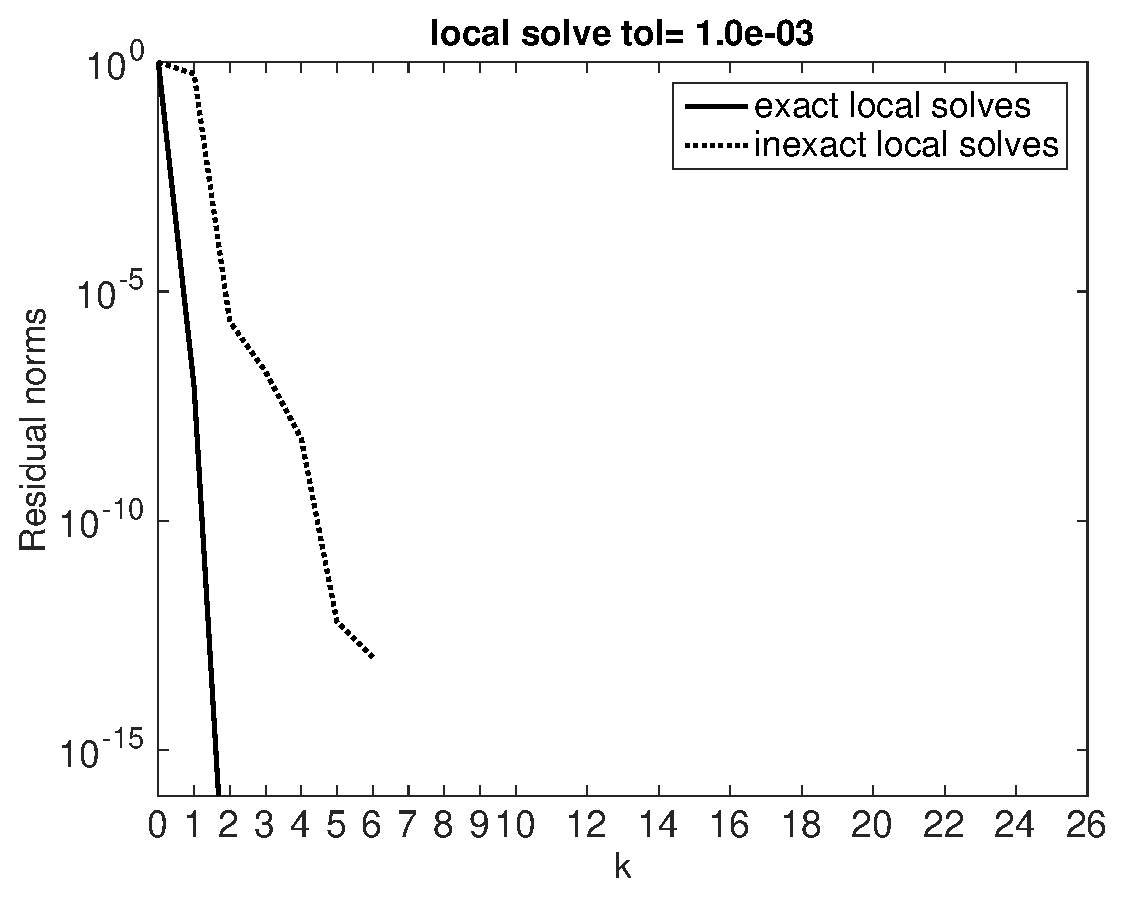
\includegraphics[width=0.98\linewidth]{figures/gmres_precond_upwind2D_eps_1e-08_inexact-1e-03_N_30_M_40}
% \end{minipage}
% %
% \begin{minipage}[t]{0.48\linewidth}
% 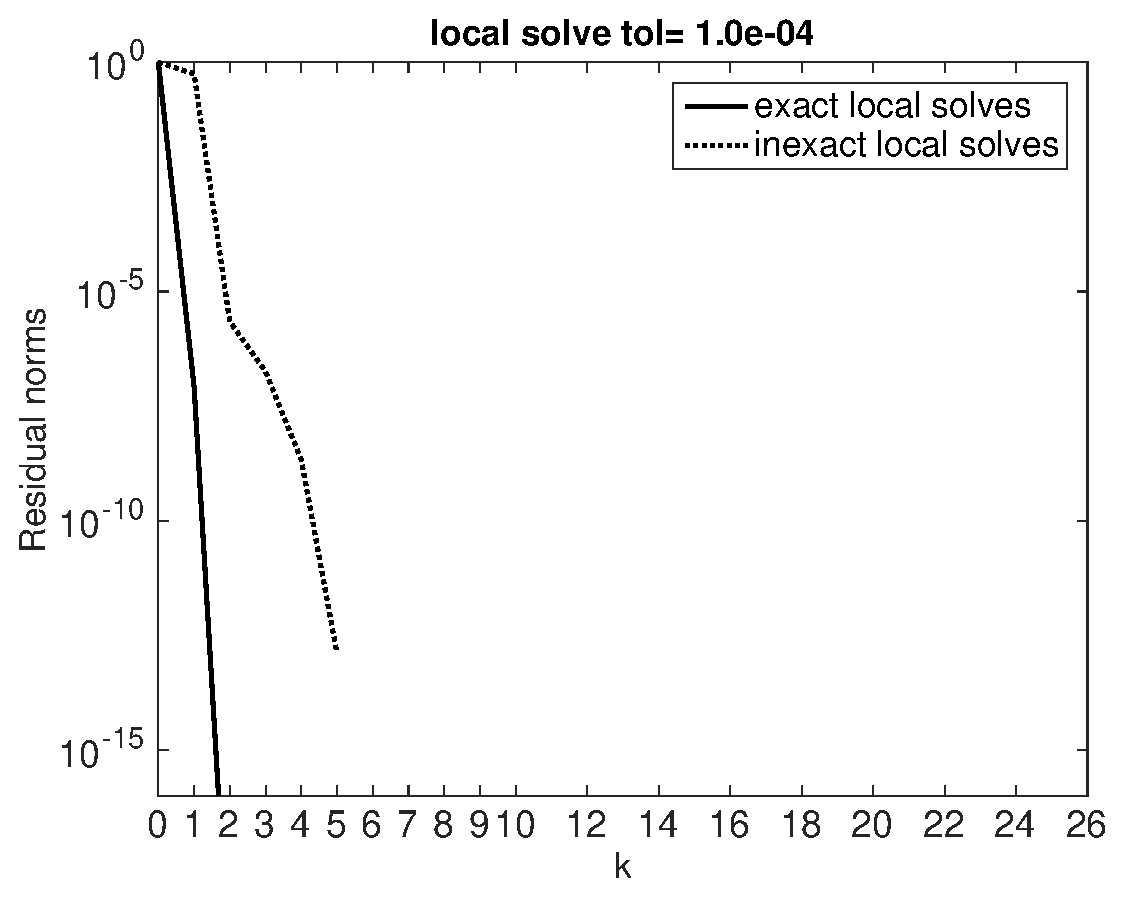
\includegraphics[width=0.98\linewidth]{figures/gmres_precond_upwind2D_eps_1e-08_inexact-1e-04_N_30_M_40}
% \end{minipage}
% \caption{Unpreconditioned and preconditioned GMRES convergence for $\epsilon~=~10^{-8}$ with inexact localsolve tolerance of $10^{-3}$ [l.] and $10^{-4}$ [r.].}
% \label{fig:2D:GMRES.inexact.prec.N30.M40.eps8.tol3_4}
% \end{figure}
%
%
% We conclude our numerical experiments by presenting
Table~\ref{tab:2D:GMRES.iter.inexact.prec} %--\ref{tab:1D:inexact_central}
shows the total number of iterations needed for the outer iteration to achieve a relative residual norm  of $10^{-7}$ when the local subdomain problems are both solved inexactly as well as exactly for different values of $\epsilon$, local solve tolerance and problem size.
%
\begin{table}[tbhp]
% \hspace*{-1.5cm}
\centering
\vspace*{-0.2em}
\begin{tabular}{r|cccccc}
%\cline{1-5}
\hline
\multicolumn{7}{c}{outer iterations [exact/inexact(inner)]}\\
\hline
\hline
\multicolumn{7}{c}{$\A\in\mathbb{R}^{1131\times1131}$}\\
\hline
\multicolumn{1}{c|}{\diagbox{$\epsilon$}{tol}} & $10^{-1}$ & $10^{-2}$ & $10^{-3}$ & $10^{-4}$ & $10^{-5}$ & $10^{-6}$\\
\hline
\multicolumn{1}{c|}{$10^{-8}$} & $1/1(2)$ & $1/1(2)$  & $1/1(2)$  & $1/1(2)$   & $1/1(2)$  & $1/1(2)$\\
\multicolumn{1}{c|}{$10^{-6}$} & $2/1(2)$ & $2/1(2)$ & $2/1(2)$  & $2/1(2)$   & $2/1(2)$  & $2/2(129)$\\
\multicolumn{1}{c|}{$10^{-4}$} & $2/1(2)$ & $2/1(2)$ & $2/1(2)$  & $2/2(132)$   & $2/2(175)$  & $2/2(195)$\\
\multicolumn{1}{c|}{$10^{-2}$} & $5/1(2)$ & $5/5(290)$ & $5/5(388)$ & $5/5(534)$ & $5/5(647)$ & $5/5(651)$\\
\hline
\hline
\multicolumn{7}{c}{$\A\in\mathbb{R}^{2891\times2891}$}\\
\hline
\multicolumn{1}{c|}{$10^{-8}$} & $2/1(2)$   & $2/1(2)$   & $2/1(2)$    & $2/1(2)$    & $2/1(2)$    & $2/1(2)$\\
\multicolumn{1}{c|}{$10^{-6}$} & $2/1(2)$   & $2/1(2)$   & $2/1(2)$    & $2/1(2)$    & $2/1(2)$    & $2/1(189)$\\
\multicolumn{1}{c|}{$10^{-4}$} & $2/1(2)$  & $2/1(2)$  & $2/1(2)$    & $2/2(196)$    & $2/2(282)$    & $2/2(288)$\\
\multicolumn{1}{c|}{$10^{-2}$} & $6/1(2)$  & $6/5(390)$ & $6/6(573)$ & $6/6(790)$ & $6/6(966)$ & $6/6(1117)$\\
\hline
\hline
\multicolumn{7}{c}{$\A\in\mathbb{R}^{4071\times4071}$}\\
\hline
\multicolumn{1}{c|}{$10^{-8}$} & $2/1(2)$   & $2/1(2)$   & $2/1(2)$    & $2/1(2)$    & $2/1(2)$    & $2/1(2)$\\
\multicolumn{1}{c|}{$10^{-6}$} & $2/1(2)$   & $2/1(2)$   & $2/1(2)$    & $2/1(2)$    & $2/1(2)$    & $2/2(219)$\\
\multicolumn{1}{c|}{$10^{-4}$} & $2/1(2)$  & $2/1(2)$  & $2/1(2)$    & $2/2(231)$    & $2/1(327)$    & $2/2(362)$\\
\multicolumn{1}{c|}{$10^{-2}$} & $6/1(2)$  & $6/5(435)$ & $6/6(637)$ & $6/6(843)$ & $6/6(1067)$ & $6/6(1240)$\\
\end{tabular}
\caption{Total iteration count for solving problem~\eqref{eq:2D:2Dbvp} using GMRES with exact and inexact Shishkin-Schwarz preconditioning to reach a relative residual norm of $10^{-7}$ for different sizes, perturbation parameters and local solve tolerances.}
\label{tab:2D:GMRES.iter.inexact.prec}
\end{table}

The results of Table~\ref{tab:2D:GMRES.iter.inexact.prec} show a surprising relation between the level of convection dominance and the accuracy of solution of the local subdomain problems. When the perturbation parameter is smaller than the local solve tolerance, the solution to the preconditioned system is reached in equal or less number of iterations than the case with exact local solves. When the local solve tolerance is chosen at the same level or smaller than the perturbation parameter the outer iterations remain less than or equal to the case with exact local solves, however, the number of inner iterations needed to solve the system increases greatly. Nevertheless, they may converge in less computational time if the saving from the inexact local solve is sufficiently large to offset the loss in convergence rate (the total computational time needed to achieve the desired solutions is shown in Table~\ref{tab:2D:GMRES.time.inexact.prec}). Another surprising feature that can be seen in Table~\ref{tab:2D:GMRES.iter.inexact.prec} is the fact that for all cases, the preconditioned GMRES method converges in at most 6 steps, when according to \eqref{eq:2D:K_rank} we would expect it to converge in the order of $N-1$ steps. Although, \eqref{eq:2D:K_rank} is an upper bound, an exploration of the singular values of the matrix $\T_{ij}$ shows that indeed the first $N$ singular values are comparable in size, however they are all one order of magnitude smaller than the the order of the perturbation parameter. Further experiments and analysis are needed to understand this phenomenon. We continue our analysis by showing the total computational time needed to reach the aforementioned solutions.

\begin{table}[tbhp]
\hspace*{-1.0cm}
\centering
\vspace*{-0.2em}
\begin{tabular}{r|ccccccccc}
%\cline{1-5}
\hline
\multicolumn{10}{c}{time [s.]}\\
\hline
\hline
\multicolumn{10}{c}{$\A\in\mathbb{R}^{1131\times1131}$}\\
\hline
% \multicolumn{2}{c|}{} & \multicolumn{1}{c|}{unpreconditioned}&\multicolumn{7}{c}{preconditioned}\\

\multicolumn{1}{c|}{$\epsilon$} & \textbackslash & unprec & exact &  $10^{-1}$ & $10^{-2}$ & $10^{-3}$ & $10^{-4}$ & $10^{-5}$ & $10^{-6}$\\
\hline
\multicolumn{1}{c|}{$10^{-8}$} & $0.0099$ & $2.5303$  & $0.0251$  & $0.0795$   & $0.0775$ & $0.0668$ & $0.0626$ & $0.0779$ & $0.0683$\\
\multicolumn{1}{c|}{$10^{-6}$} & $0.0110$ & $2.6841$  & $0.0264$  & $0.0602$   & $0.0719$ & $0.0716$ & $0.0561$ & $0.0797$ & $0.3162$\\
\multicolumn{1}{c|}{$10^{-4}$} & $0.0107$ & $2.5351$  & $0.0265$  & $0.0718$   & $0.0765$ & $0.0602$ & $0.3244$ & $0.3952$ & $0.4441$\\
\multicolumn{1}{c|}{$10^{-2}$} & $0.0111$ & $1.1483$  & $0.0371$  & $0.0536$   & $0.6477$ & $0.8750$ & $1.1159$ & $1.3260$ & $1.3568$\\
\hline
\hline
\multicolumn{10}{c}{$\A\in\mathbb{R}^{2891\times2891}$}\\
\hline
\multicolumn{1}{c|}{$10^{-8}$} & $0.0384$ & $25.2496$  & $0.3096$  & $0.3108$   & $0.2579$ & $0.2747$ & $0.3008$ & $0.3258$ & $0.2869$\\
\multicolumn{1}{c|}{$10^{-6}$} & $0.0432$ & $30.6092$  & $0.1846$  & $0.2579$   & $0.2447$ & $0.2833$ & $0.2490$ & $0.2553$ & $1.8440$\\
\multicolumn{1}{c|}{$10^{-4}$} & $0.0285$ & $25.1235$  & $0.2372$  & $0.2640$   & $0.2680$ & $0.2472$ & $1.5442$ & $2.0936$ & $2.1142$\\
\multicolumn{1}{c|}{$10^{-2}$} & $0.0299$ & $5.3121$  & $0.2377$  & $0.2427$   & $2.9197$ & $4.0689$ & $5.5994$ & $6.7012$ & $7.9111$\\
\hline
\hline
\multicolumn{10}{c}{$\A\in\mathbb{R}^{4071\times4071}$}\\
\hline
\multicolumn{1}{c|}{$10^{-8}$} & $0.0531$ & $99.6026$  & $0.6738$  & $0.5405$   & $0.5991$ & $0.6309$  & $0.6762$  & $0.6097$  & $0.5066$\\
\multicolumn{1}{c|}{$10^{-6}$} & $0.0450$ & $92.4812$  & $0.4906$  & $0.4900$   & $0.4881$ & $0.5883$  & $0.4675$  & $0.4564$  & $2.9675$\\
\multicolumn{1}{c|}{$10^{-4}$} & $0.0554$ & $90.0034$  & $0.4219$  & $0.8435$   & $0.4765$ & $0.5237$  & $3.2154$  & $4.3034$  & $4.7171$\\
\multicolumn{1}{c|}{$10^{-2}$} & $0.0721$ &  $13.2551$  & $0.6031$  &  $0.4286$   & $5.5991$ & $7.9189$ & $10.2299$ & $12.9283$ & $15.1270$\\
\end{tabular}
\caption{Total CPU time for solving problem~\eqref{eq:2D:2Dbvp} with \texttt{MATLAB}'s backslash and GMRES with and without Shishkin-Schwarz preconditioning for different problem sizes. Timings are reported for GMRES to reach a relative residual norm of $10^{-7}$ with exact and inexact preconditioning.}
\label{tab:2D:GMRES.time.inexact.prec}
\end{table}

Table~\ref{tab:2D:GMRES.time.inexact.prec} shows that for all the problem sizes chosen for the experiments, the backslash solution is obtained very fast while the unpreconditioned GMRES method is very slow with increasing time as the convection dominance increases. As the problem size increases, the performance of GMRES deteriorates greatly, showing that for a much larger number of unknowns (when the backslash solution is no longer available) and a very small perturbation parameter, the unpreconditioned GMRES will very likely be innefficient. For the preconditioned system with exact local solves this is not the case, although still one order of magnitude slower than the backslash solution, we can see a more or less constant solution time for different values of the perturbation parameter. The benefits of the inexact local solve approach is shown by comparing the time it takes for the unpreconditioned GMRES method with any of the inexact local solve times -  the speed up is always greater than three orders of magnitude, even for the case of a very low local solve tolerance.
%
\begin{figure}[h!]
\hspace{-1cm}
\centering
\begin{minipage}[t]{0.99\linewidth}
\centering
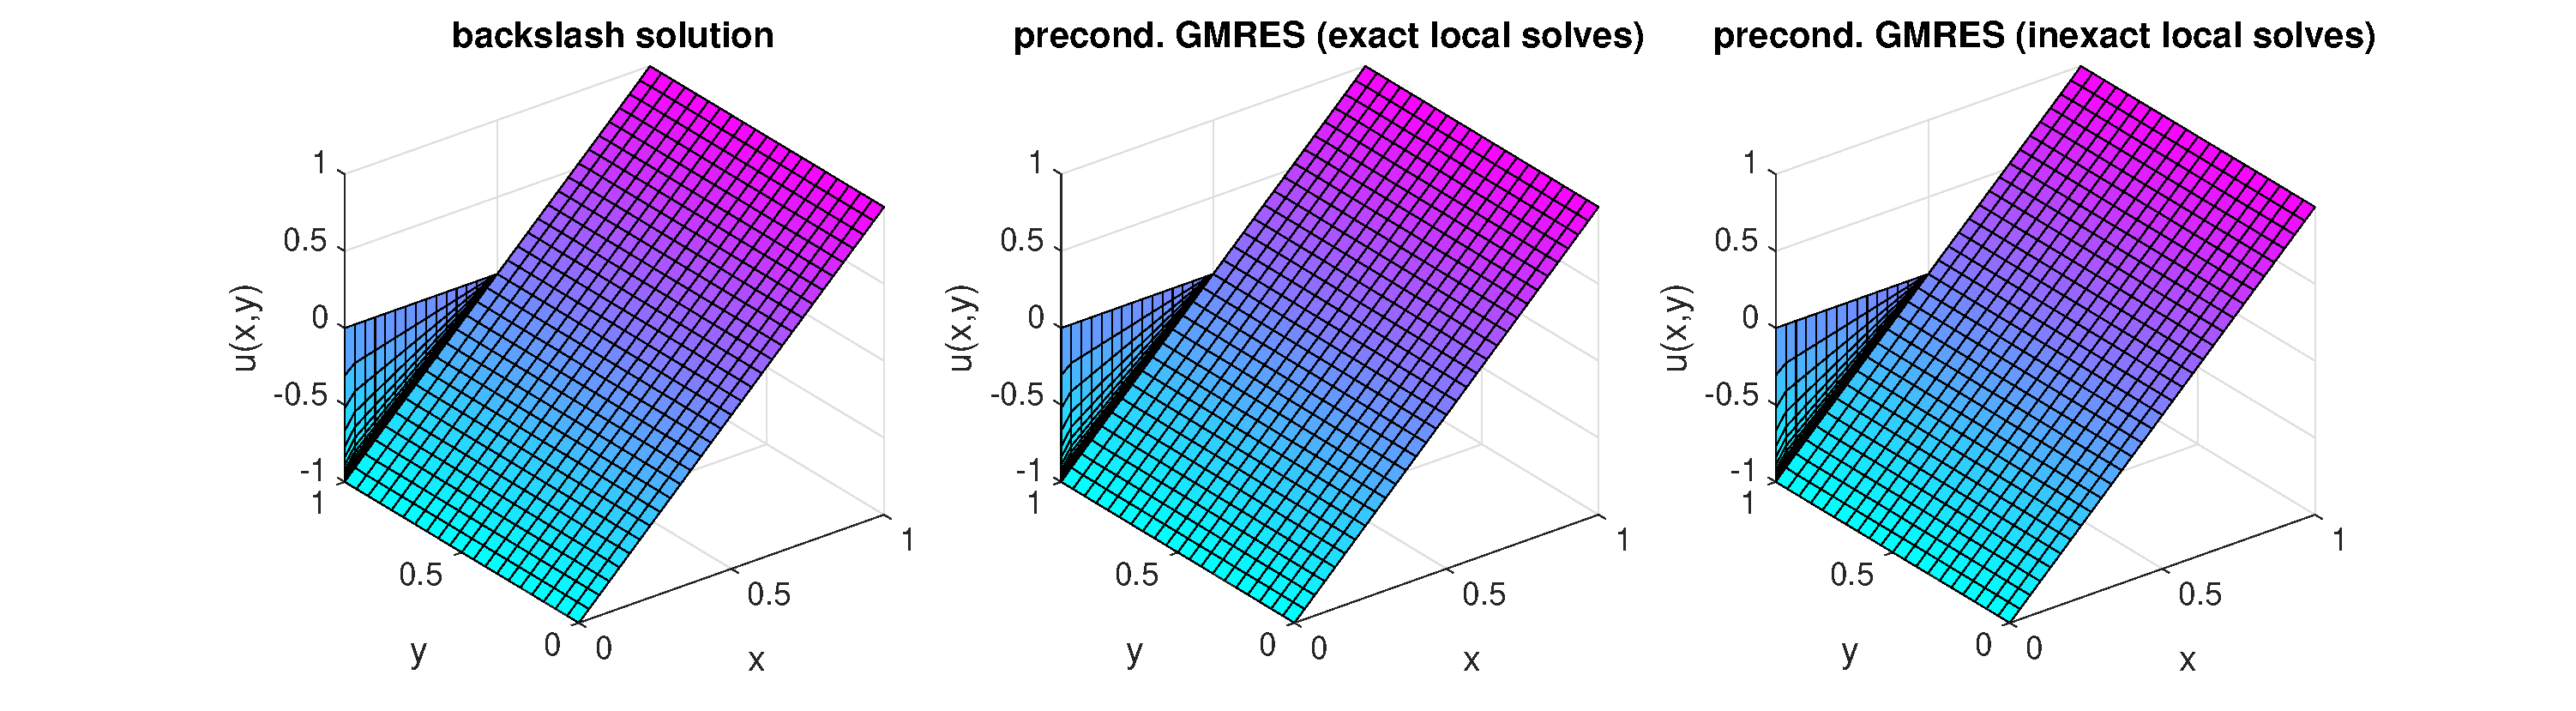
\includegraphics[width=0.98\linewidth]{figures/sol_comp}
\end{minipage}
\caption{Comparison of obtained solutions for $N=30$, $M=40$, $\epsilon~=~10^{-8}$ and inexact local solve tolerance of $10^{-1}$.}
\label{fig:2D:sol_comp}
\end{figure}

For the specific case of $\epsilon=10^{-8}$, $N=30$ and $M=40$,
Figure~\ref{fig:2D:sol_comp} shows a comparison of the obtained solutions for
the exact case (backslash solution of \eqref{eq:2D:linsys}), and the cases of
solving the preconditioned system with exact and inexact local solves (GMRES
solution of \eqref{eq:2D:precond}) with a tolerance of $10^{-1}$. The accuracy
of the obtained solutions is presented in
Table~\ref{tab:2D:GMRES.error.inexact.prec}, which shows the relative normwise
error of the obtained solutions with respect to the exact solution obtained
with the backslash operator for all the experiments presented in
Tables~\ref{tab:2D:GMRES.iter.inexact.prec} and \ref{tab:2D:GMRES.time.inexact.prec}.

\begin{table}[tbhp]
\hspace*{-2.5cm}
\centering
\vspace*{-0.2em}
\begin{tabular}{r|cccccccc}
%\cline{1-5}
\hline
\multicolumn{9}{c}{relative error [$\|\u_{*}-\u_{\textbackslash}\|/\|\u_{\textbackslash}\|$]}\\
\hline
\hline
\multicolumn{9}{c}{$\A\in\mathbb{R}^{1131\times1131}$}\\
\hline
\multicolumn{1}{c|}{$\epsilon$} & $\u_{unprec}$ & $\u_{exact}$ & $\u_{10^{-1}}$ & $\u_{10^{-2}}$ & $\u_{10^{-3}}$ & $\u_{10^{-4}}$ & $\u_{10^{-5}}$ & $\u_{10^{-6}}$\\
\hline
\multicolumn{1}{c|}{$10^{-8}$} & $3.5\times10^{-7}$ & $8.4\times10^{-8}$  & $1.2\times10^{-7}$  & $1.2\times10^{-7}$   & $1.2\times10^{-7}$ & $1.2\times10^{-7}$  & $1.2\times10^{-7}$  & $1.2\times10^{-7}$ \\
\multicolumn{1}{c|}{$10^{-6}$} & $2.8\times10^{-9}$ & $7.2\times10^{-15}$  & $1.2\times10^{-5}$  & $1.2\times10^{-5}$   & $1.2\times10^{-5}$ & $1.2\times10^{-5}$  & $1.2\times10^{-5}$   & $2.8\times10^{-10}$ \\
\multicolumn{1}{c|}{$10^{-4}$} & $3.5\times10^{-11}$ & $7.7\times10^{-9}$  & $1.2\times10^{-3}$  & $1.2\times10^{-3}$   & $1.2\times10^{-3}$ & $2.8\times10^{-6}$  & $2.8\times10^{-6}$   & $2.3\times10^{-6}$ \\
\multicolumn{1}{c|}{$10^{-2}$} & $3.5\times10^{-13}$ & $3.6\times10^{-8}$  & $8.8\times10^{-2}$  & $2.1\times10^{-2}$   & $2.7\times10^{-3}$ & $2.8\times10^{-4}$  & $2.4\times10^{-5}$   & $2.1\times10^{-6}$ \\
\hline
\hline
\multicolumn{9}{c}{$\A\in\mathbb{R}^{2891\times2891}$}\\
\hline
\multicolumn{1}{c|}{$10^{-8}$} & $1.9\times10^{-6}$ & $1.0\times10^{-14}$  & $1.8\times10^{-7}$  & $1.8\times10^{-7}$   & $1.8\times10^{-7}$ & $1.8\times10^{-7}$  & $1.8\times10^{-7}$   & $1.8\times10^{-7}$ \\
\multicolumn{1}{c|}{$10^{-6}$} & $9.1\times10^{-9}$ & $2.8\times10^{-14}$  & $1.8\times10^{-5}$  & $1.8\times10^{-5}$   & $1.8\times10^{-5}$ & $1.8\times10^{-5}$  & $1.8\times10^{-5}$   & $6.6\times10^{-10}$ \\
\multicolumn{1}{c|}{$10^{-4}$} & $8.5\times10^{-11}$ & $2.7\times10^{-8}$  & $1.8\times10^{-3}$  & $1.8\times10^{-3}$   & $1.8\times10^{-3}$ & $6.6\times10^{-6}$  & $6.6\times10^{-6}$   & $5.7\times10^{-8}$ \\
\multicolumn{1}{c|}{$10^{-2}$} & $1.1\times10^{-12}$ & $1.7\times10^{-8}$  & $1.3\times10^{-1}$  & $3.1\times10^{-2}$   & $3.4\times10^{-3}$ & $4.0\times10^{-4}$  & $3.2\times10^{-5}$   & $4.9\times10^{-6}$ \\
\hline
\hline
\multicolumn{9}{c}{$\A\in\mathbb{R}^{4071\times4071}$}\\
\hline
\multicolumn{1}{c|}{$10^{-8}$} & $3.6\times10^{-6}$ & $1.0\times10^{-14}$  & $2.1\times10^{-7}$  & $2.1\times10^{-7}$   & $2.1\times10^{-7}$ & $2.1\times10^{-7}$  & $2.1\times10^{-7}$   & $2.1\times10^{-7}$ \\
\multicolumn{1}{c|}{$10^{-6}$} & $1.3\times10^{-8}$ & $4.6\times10^{-14}$  & $2.1\times10^{-5}$  & $2.1\times10^{-5}$   & $2.1\times10^{-5}$ & $2.1\times10^{-5}$  & $2.1\times10^{-5}$   & $9.1\times10^{-10}$ \\
\multicolumn{1}{c|}{$10^{-4}$} & $1.8\times10^{-10}$ & $4.1\times10^{-8}$  & $2.1\times10^{-3}$  & $2.1\times10^{-3}$   & $2.1\times10^{-3}$ & $9.1\times10^{-6}$  & $9.1\times10^{-6}$   & $9.5\times10^{-8}$ \\
\multicolumn{1}{c|}{$10^{-2}$} & $1.9\times10^{-12}$ & $4.2\times10^{-8}$  & $1.4\times10^{-1}$  & $4.0\times10^{-2}$   & $5.2\times10^{-3}$ & $4.7\times10^{-4}$  & $5.2\times10^{-5}$   & $6.1\times10^{-6}$ \\
\end{tabular}
\caption{Relative error $\|\u_{*}-\u_{\textbackslash}\|/\|\u_{\textbackslash}\|$, with $\|\cdot\|=\|\cdot\|_{2}$ for each solution approach}
\label{tab:2D:GMRES.error.inexact.prec}
\end{table}
\pagebreak
For a fixed level of convection dominance ($\epsilon$), Table~\ref{tab:2D:GMRES.error.inexact.prec} shows that, on the one hand,  solving the preconditioned system with exact local solves delivers a more accurate solution than solving the unpreconditioned system using GMRES when the convection dominance is high (less than $10^{-4}$) and the opposite is true for low convection dominance (comparison of columns 1 \& 2). Furthermore, solving the system with inexact local solves always delivers a less accurate solution (at least one order of magnitude worse) than using exact local solves, neverthless, the difference diminishes as the convection dominance is increased (comparison of column 2 with columns 3-7).




% Table~\ref{tab:2D:GMRES.inexact.prec.1} shows the number of outer iterations as well as the total time needed for GMRES to achieve convergence for both the case of exact and the case of inexact local solves for a problem with $N=50$ and $M=60$.



% \section*{{\textcolor{white}{ghost}}}
% \label{sec:ghost}
% \subsection*{{\textcolor{white}{ghost2}}}

\fi
